\documentclass[11pt,a4paper]{article}
\usepackage[T1]{fontenc}
\usepackage[utf8]{inputenc}
\usepackage{lmodern}
\usepackage[margin=1in]{geometry}
\usepackage{microtype}
\usepackage{hyperref}
\usepackage{graphicx}
\usepackage[space]{grffile}      % allow spaces in file names for \includegraphics
\usepackage{xstring}             % string tests for filename-based sizing
\usepackage{siunitx}             % for \SI{..}{MB} etc.
\usepackage{caption}
\captionsetup{font=small}
\usepackage{setspace}
\usepackage{titlesec}
\usepackage{xcolor}
\usepackage{hyperref}
\usepackage{enumitem}
\usepackage{graphicx}
\usepackage{booktabs}
\usepackage{listings}
\usepackage{caption}
\usepackage{minted}
\usepackage{siunitx}
\usepackage{graphicx}
\usepackage[space]{grffile}

\newcommand{\locustwide}[1]{\includegraphics[width=.55\linewidth]{#1}}
\newcommand{\locustnarrow}[1]{\includegraphics[width=.45\linewidth]{#1}}
\newcommand{\lambdawide}[1]{\includegraphics[width=.92\linewidth]{#1}}
\newcommand{\lambdahalf}[1]{\includegraphics[width=.70\linewidth]{#1}}


\hypersetup{
  colorlinks=true,
  linkcolor=black,
  urlcolor=blue,
  citecolor=black,
  pdfauthor={<Your Name>},
  pdftitle={Serverless Named Entity Recognition on AWS Lambda},
  pdfsubject={Cloud Computing Project Report},
  pdfkeywords={AWS Lambda, API Gateway, SAM, spaCy, NER, Serverless, CloudWatch, Locust}
}

\lstdefinestyle{code}{
  basicstyle=\ttfamily\small,
  keywordstyle=\bfseries\color{black},
  commentstyle=\itshape\color{gray!70!black},
  stringstyle=\color{teal!60!black},
  showstringspaces=false,
  frame=single,
  framerule=0.3pt,
  rulecolor=\color{black!20},
  breaklines=true,
  columns=fullflexible
}
\lstset{style=code}

\makeatletter
\let\orig@includegraphics\includegraphics
\renewcommand{\includegraphics}[2][]{%
  \begingroup
    \def\imgfile{#2}%
    % Locust - Charts
    \IfSubStr{\imgfile}{Charts}{%
      \orig@includegraphics[width=.55\linewidth]{#2}%
    }{%
      % Locust - Stats
      \IfSubStr{\imgfile}{Stats}{%
        \orig@includegraphics[width=.45\linewidth]{#2}%
      }{%
        % Lambda metrics
        \IfSubStr{\imgfile}{Duration}{%
          \orig@includegraphics[width=.70\linewidth]{#2}%
        }{%
          \IfSubStr{\imgfile}{Invocation}{%
            \orig@includegraphics[width=.70\linewidth]{#2}%
          }{%
            \IfSubStr{\imgfile}{Invocations}{%
              \orig@includegraphics[width=.70\linewidth]{#2}%
            }{%
              \IfSubStr{\imgfile}{Concurrent}{%
                \orig@includegraphics[width=.70\linewidth]{#2}%
              }{%
                \IfSubStr{\imgfile}{ConcEx}{%
                  \orig@includegraphics[width=.70\linewidth]{#2}%
                }{%
                  % default
                  \orig@includegraphics[width=\linewidth]{#2}%
                }%
              }%
            }%
          }%
        }%
      }%
    }%
  \endgroup
}
\makeatother

\title{\vspace{-1.5em}\Large\bfseries Serverless Named Entity Recognition on AWS Lambda}
\author{Riccardo Pitzanti - 1947877 \quad \quad \quad \quad Federico Iannini - 1931748\\
  \normalsize pitzanti.1947877@studenti.uniroma1.it \quad iannini.1931748@studenti.uniroma1.it\\[0.25em]
  \normalsize Sapienza Università di Roma}
\date{\normalsize \today}

\begin{document}
\maketitle
\vspace{-1.5em}

\section{Introduction}
The proliferation of unstructured textual data across digital platforms has precipitated a growing demand for efficient and scalable information extraction techniques. Named Entity Recognition (NER), a fundamental subtask within Natural Language Processing (NLP), serves as a critical enabling technology for this purpose, tasked with identifying and classifying atomic elements in text into predefined categories such as persons, organizations, and locations. The operationalization of such NLP models, however, traditionally necessitates managing server infrastructure, which introduces complexity, overhead, and potential underutilization of resources.

This work explores the application of a serverless computing paradigm to address these challenges, deploying a production-ready NLP pipeline for NER on AWS Lambda. By leveraging AWS Lambda and Amazon API Gateway, we architect a microservice that is inherently scalable, cost-efficient, and devoid of server management concerns. The implementation utilizes the spaCy library, a robust industrial-strength framework for NLP in Python, ensuring high-quality inference capabilities. The entire application stack—including compute, API management, and security—is defined and deployed programmatically using the AWS Serverless Application Model (SAM), embodying Infrastructure-as-Code (IaC) principles to guarantee reproducibility and reliability.

The primary objective of this study is to design, implement, and rigorously evaluate the performance characteristics of this serverless NER service under varied load conditions. We employ Locust, an open-source load-testing tool, to simulate traffic patterns ranging from benign to stressful, measuring key client-side and provider-side metrics. Our analysis focuses on quantifying latency, throughput, stability, and the impact of vertical scaling (memory allocation) within the constraints of an educational AWS environment. The findings demonstrate the viability of serverless architectures for deploying lightweight, performant, and cost-effective NLP microservices.

\section{Background}

\subsection{Named Entity Recognition (NER) and spaCy}
Named Entity Recognition (NER) is a natural language processing (NLP) task focused on identifying and categorizing information elements, known as entities, within unstructured text. These entities are typically classified into predefined categories such as persons (\textsf{PERSON}), organizations (\textsf{ORG}), and geopolitical entities (\textsf{GPE}). The spaCy library in Python provides a production-ready framework for implementing NLP pipelines, offering statistical models for tasks like NER.

\subsection{AWS SAM \& Containerized Build with Docker}
The AWS Serverless Application Model (SAM) is an open-source framework that extends AWS CloudFormation to provide a simplified syntax for defining serverless resources. It is a form of Infrastructure as Code (IaC) specifically designed to express the functions, APIs, permissions, and events that compose a serverless application. A containerized build process involves using a consistent, isolated environment to compile application dependencies and package the code. By employing Docker, SAM ensures that the build process is executed within a containerized environment that replicates the AWS Lambda runtime. This guarantees consistency between the development build and the deployment target, thereby mitigating compatibility issues.

\subsection{AWS Lambda and HTTP API}
AWS Lambda is a serverless, event-driven compute service that allows for the execution of code in response to triggers without requiring the management of underlying servers. It automatically scales with incoming request volume and utilizes a fine-grained cost model based on actual compute consumption. The Amazon API Gateway is a fully managed service that simplifies the creation, publication, and maintenance of secure APIs at any scale. It acts as a front-door for applications to access data and business logic from backend services, providing essential features like HTTP endpoint management, request routing, and authorization.

\subsection{Observability with CloudWatch}
Observability is a system property that describes how well internal states can be understood from external outputs, primarily through the collection and analysis of logs, metrics, and traces. Amazon CloudWatch is a monitoring and observability service that provides a unified view of AWS resource health, application performance, and operational trends. It automatically collects performance metrics from services like AWS Lambda.

\subsection{Load Testing with Locust}
Locust is an open-source load testing tool that allows developers to define user behavior with Python code and simulate various concurrent users to assess a system's performance under stress. Its distributed and scalable nature makes it suitable for testing the limits of web services and APIs. It provides a real-time web-based user interface to visualize performance indicators such as requests per second, response times, and the number of failing requests as the test is running.

\section{System Design and Implementation}
\subsection{Architecture overview}
\begin{itemize}[leftmargin=1.3em]
  \item \textbf{Client} sends \texttt{POST /ner} with a short text body.
  \item \textbf{API Gateway (HTTP API)} forwards requests to Lambda.
  \item \textbf{Lambda} parses input, runs spaCy NER (warm model), and returns spans.
  \item \textbf{CloudWatch} records metrics and logs for observability.
\end{itemize}

\noindent\textbf{API contract.}
\begin{minted}[
    frame=single,
    linenos
  ]{json}
POST /ner
Content-Type: application/json
{"text": "Alan Turing was born on June 23, 1912, in London, England."}

200 OK
{"entities": [
    {'text': 'Alan Turing', 'label': 'PERSON', 'start': 0, 'end': 11},
    {'text': 'June 23, 1912', 'label': 'DATE', 'start': 24, 'end': 37},
    {'text': 'London', 'label': 'GPE', 'start': 41, 'end': 47},
    {'text': 'England', 'label': 'GPE', 'start': 49, 'end': 56}]
}
\end{minted}
%caption={Request and response schemas (illustrative).}


\section{Methodology and Implementation}

\subsection{Inference Core Module (\texttt{src/ner.py})}
This module constitutes the computational core responsible for the Named Entity Recognition (NER) task. It utilizes the spaCy library, a framework for natural language processing (NLP) in Python. The pre-trained statistical model (\texttt{en\_core\_web\_sm}) is loaded into a global constant at module import time. The primary function, \texttt{extract\_entities(text: str)}, processes an input string through the spaCy pipeline. It returns a list of dictionaries, each containing the extracted entity's surface form (\texttt{text}), its ontological class (\texttt{label}), and the character-level indices (\texttt{start}, \texttt{end}) denoting its span within the original text.

\subsection{Lambda Handler Function (\texttt{src/handler.py})}
This module implements the AWS Lambda function handler, which serves as the entry point for requests proxied by Amazon API Gateway. Its primary role is to manage the HTTP request-response cycle. The handler first invokes a helper function, \texttt{\_parse\_body}, to normalize the incoming event structure. This function abstracts away the differences between the event payload delivered by API Gateway (where the HTTP request body is passed as a JSON-encoded string) and the event object used during local testing (which may be a Python dictionary). The handler then performs input validation, checking for the presence and type of the required \texttt{'text'} field. Invalid requests result in a \texttt{400 Bad Request} response. Validated text is passed to the inference core, and the resulting entities are serialized into a JSON object returned within a \texttt{200 OK} response, complete with appropriate HTTP headers for content type.

\subsection{Build Process}
The build is executed using the AWS SAM CLI command \texttt{sam build --use-container}. This process constructs the deployment package inside a Docker container that emulates the Amazon Linux environment of AWS Lambda.

\subsection{Infrastructure Provisioning (SAM Template)}
The cloud infrastructure is defined declaratively using the AWS Serverless Application Model (SAM), an extension of AWS CloudFormation. The template, \texttt{template.yaml}, specifies a minimal and functional stack:
\begin{itemize}
    \item A single AWS Lambda function resource with its runtime (\texttt{python3.9}), allocated memory (512 MB), and timeout (15 seconds) defined in the \texttt{Globals} section.
    \item An Amazon API Gateway HTTP API resource, which provisions a managed HTTPS endpoint. This API is configured with a single route (\texttt{POST /ner}) that integrates directly with the Lambda function.
    \item A pre-existing IAM role (\texttt{LabRole}) is referenced for execution permissions, a constraint of the AWS Academy Learner Lab environment. In a standard AWS account, SAM would typically generate a minimal role with necessary permissions automatically.
\end{itemize}
This Infrastructure-as-Code (IaC) approach guarantees that the entire application stack is versioned, reproducible, and deployable with a single command.

\subsection{Front-End}
The front-end component of the application is deliberately designed as a minimal web interface to facilitate testing and demonstration of the deployed Named Entity Recognition (NER) service. It is implemented as a static \texttt{HTML} page enriched with basic \texttt{JavaScript} logic. The interface provides a text area where the user can enter arbitrary input and a form field for specifying the API Gateway endpoint generated during the deployment process. Upon submission, the client-side script performs an asynchronous \texttt{HTTP POST} request to the NER API, transmitting the input text in JSON format.

The server's response, which consists of the extracted named entities together with their associated labels, is rendered directly in the browser in a structured JSON format. This design ensures transparency of the system's behavior and allows the user to validate the correctness of the back-end inference in real time.

For ease of distribution and reproducibility, the static front-end is packaged within a lightweight Docker container based on the \texttt{nginx} web server. This container exposes the page on a local port, enabling researchers and practitioners to access the interface through a standard web browser without the need for additional configuration or build tools. Such a containerized approach guarantees consistency across different environments, while maintaining the simplicity appropriate for an internal testing utility rather than a production-grade user interface.

\section{Performance Evaluation and Testing}\label{sec:testing}

\subsection{Goals and approach}
The objective is to evaluate the responsiveness, scalability, and stability of the NER microservice deployed on AWS Lambda behind an HTTP API. Each experiment uses a structured workload with \emph{Warm-up (WU)}, \emph{Ramp-up (RU)}, \emph{Steady (S)}, and \emph{Ramp-down (RD)} phases. We collect both \emph{user-oriented} (client) and \emph{system-oriented} (provider) metrics and align the CloudWatch time windows with the Locust test window (WU excluded).

\subsection{System under test (SUT) and constraints !TODO}
\begin{itemize}
  \item \textbf{Function:} AWS Lambda (Python\,3.10), NER inference (ONNXRuntime), Region \texttt{us-east-1}.
  \item \textbf{Memory:} Baseline \SI{512}{MB}; Heavy variants at \SI{1024}{MB}. We also re-ran Scenario~B Heavy at \SI{512}{MB} to assess vertical scaling (\SI{512}\,$\rightarrow$\,\SI{1024}{MB}).
  \item \textbf{API:} AWS HTTP API (API Gateway) fronting the Lambda function.
  \item \textbf{Client:} Locust on a developer workstation; single generator node.
  \item \textbf{Lab limits:} Learner Lab Lambda concurrency $\approx$ 10; budget is pay-per-request, so short, repeated runs are preferred.
\end{itemize}

\subsection{Common settings across all scenarios !TODO}
\begin{itemize}
  \item \textbf{Warm-up (WU):} \SI{60}{s} at 2 users (spawn rate 2/s) to trigger cold starts. Immediately after WU the client statistics are reset so that RU/S/RD are isolated in the reported numbers.
  \item \textbf{Payload mix:} Short and long English sentences with named entities (persons, organizations, locations, dates). Requests are \texttt{POST /ner} with a small JSON body.
  \item \textbf{Light vs Heavy:} Each scenario has a \emph{Light} profile (lower RPS) and a \emph{Heavy} profile (higher RPS). Heavy runs use near-zero client think time to approach the Lambda concurrency ceiling; Light runs use more realistic user pacing.
  \item \textbf{Timing windows:} For each run we record absolute UTC start/end times; CloudWatch queries use the same window (WU excluded) to export provider metrics.
\end{itemize}

\subsection{Workload scenarios !TODO motivate}
We use three canonical shapes; durations below refer to the \emph{main window} (after WU and stats reset). ``Users'' are active virtual users; RPS emerges from users, client think time, and function latency.

\paragraph{Scenario A — Bursty}
\begin{itemize}
  \item \textbf{Light A:} constant 5 users for \SI{300}{s}; long think time (5–10\,s) to emulate intermittent clicks $\Rightarrow$ low, flat RPS plateau.
  \item \textbf{Heavy A:} constant 10 users for $\approx$\SI{360}{s}; near-zero think time (0–0.1\,s) to drive high RPS until bounded by Lambda concurrency.
\end{itemize}

\paragraph{Scenario B — Ramp $\rightarrow$ Steady $\rightarrow$ Ramp-down !TODO CHANGE}
\begin{itemize}
  \item \textbf{Light B:} RU in \SI{60}{s} steps through 1$\rightarrow$3$\rightarrow$5$\rightarrow$6$\rightarrow$7$\rightarrow$8 users, then S at 8 users for \SI{240}{s}, then RD 4 users (\SI{60}{s}) and 1 user (\SI{60}{s}). Think time short (0.2–1.0\,s).
  \item \textbf{Heavy B:} Faster RU to 10 users, S at 10 users for $\approx$\SI{240}{s}, then RD; near-zero think time (0–0.1\,s) for high RPS.
  \item \textbf{Vertical scaling:} We executed Heavy~B twice with identical shape, once at \SI{512}{MB} and once at \SI{1024}{MB}, to quantify the impact of memory on latency (p95/p99) and steady-state throughput.
\end{itemize}

\paragraph{Scenario C — Spike}
\begin{itemize}
  \item \textbf{Light C:} pre-spike \SI{30}{s} at 1 user, spike to 8 users for \SI{240}{s}, then \SI{60}{s} at 2 users; short think time (0.2–1.0\,s).
  \item \textbf{Heavy C:} pre-spike \SI{30}{s} at 2 users, spike to 10 users for \SI{240}{s}, then \SI{60}{s} at 2 users; near-zero think time (0–0.1\,s).
\end{itemize}

\subsection{Metrics collected}
\textbf{Client (user-oriented, Locust):}
\begin{itemize}
  \item Per-run CSV/HTML with request counts, failure rate, response-time distribution (p50/p95/p99), and effective RPS during RU/S/RD (WU excluded).
\end{itemize}
\textbf{Provider (system-oriented, CloudWatch / Lambda):}
\begin{itemize}
  \item \emph{Duration} (we use p95), \emph{Invocations}, \emph{ConcurrentExecutions}.
  \item Metrics are exported at \SI{60}{s} resolution using the exact Locust main-window timestamps.
\end{itemize}

\subsection{Test variants covered in this study !TODO table}
\begin{itemize}
  \item \textbf{A, B, C (Light):} realistic pacing, lower RPS.
  \item \textbf{A, B, C (Heavy @ \SI{1024}{MB}):} near-zero think time to stress concurrency and throughput.
  \item \textbf{Vertical scaling (B Heavy, \SI{512}{MB} vs \SI{1024}{MB}):} identical shape and pacing, only the Lambda memory differs.
\end{itemize}

\section{Results and discussion !TODO enlarge images}

In this section we report the outcomes of the experiments defined in the previous section. For each scenario (A, B, C) we present both the \emph{Light} (lower RPS) and \emph{Heavy} (higher RPS) variants.

\subsection{Scenario A (Bursty)}\label{subsec:resA}

\paragraph{Light A (intermittent pacing).}
With long think times (5--10\,s) and a constant small user pool, the overall throughput remains intentionally low and flat. This profile emulates intermittent human activity rather than throughput saturation. Lambda metrics show a correspondingly low and steady invocation rate and a shallow concurrent-executions curve.

\begin{figure}[h!] \centering
  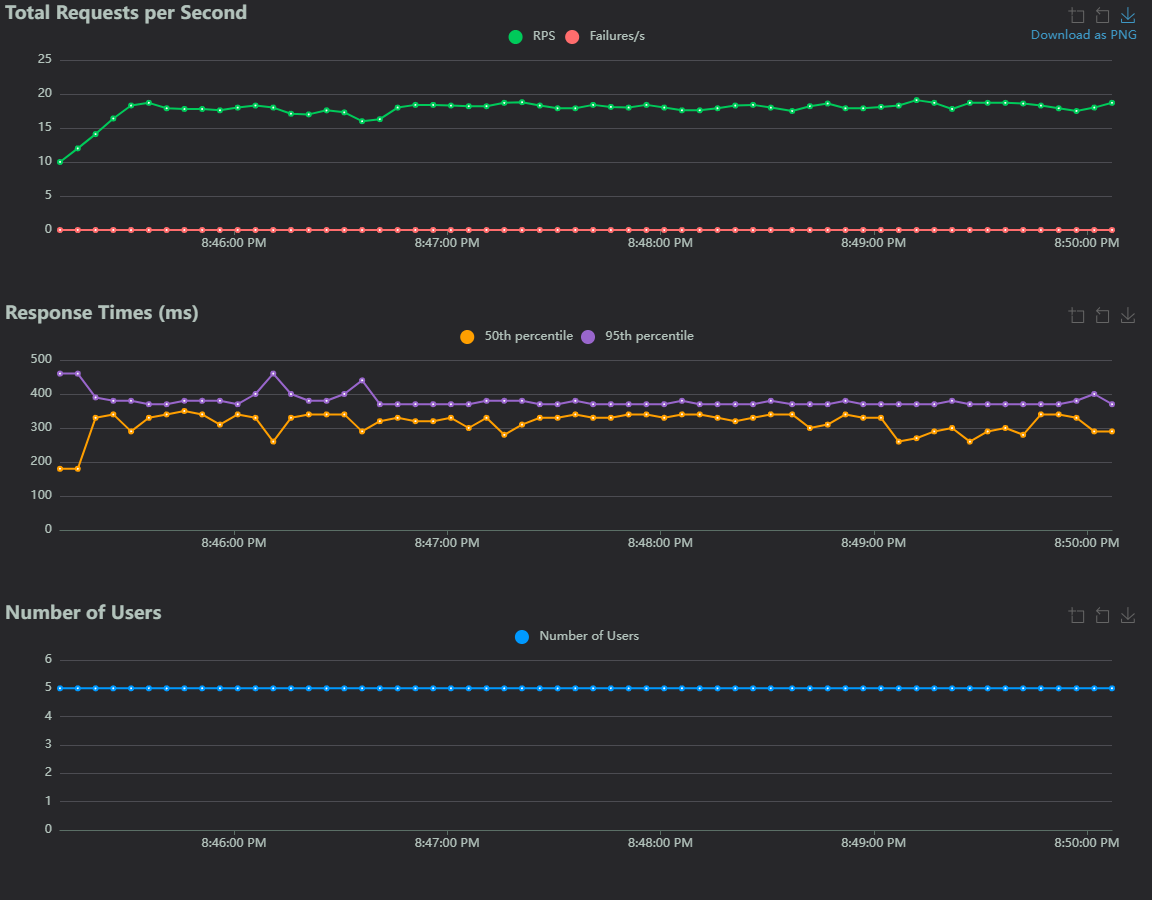
\includegraphics[width=\linewidth]{"figures/lA - Charts.png"}
  \caption{Light A --- Locust charts (overall latency/RPS).}
\end{figure}

\begin{figure}[h!] \centering
  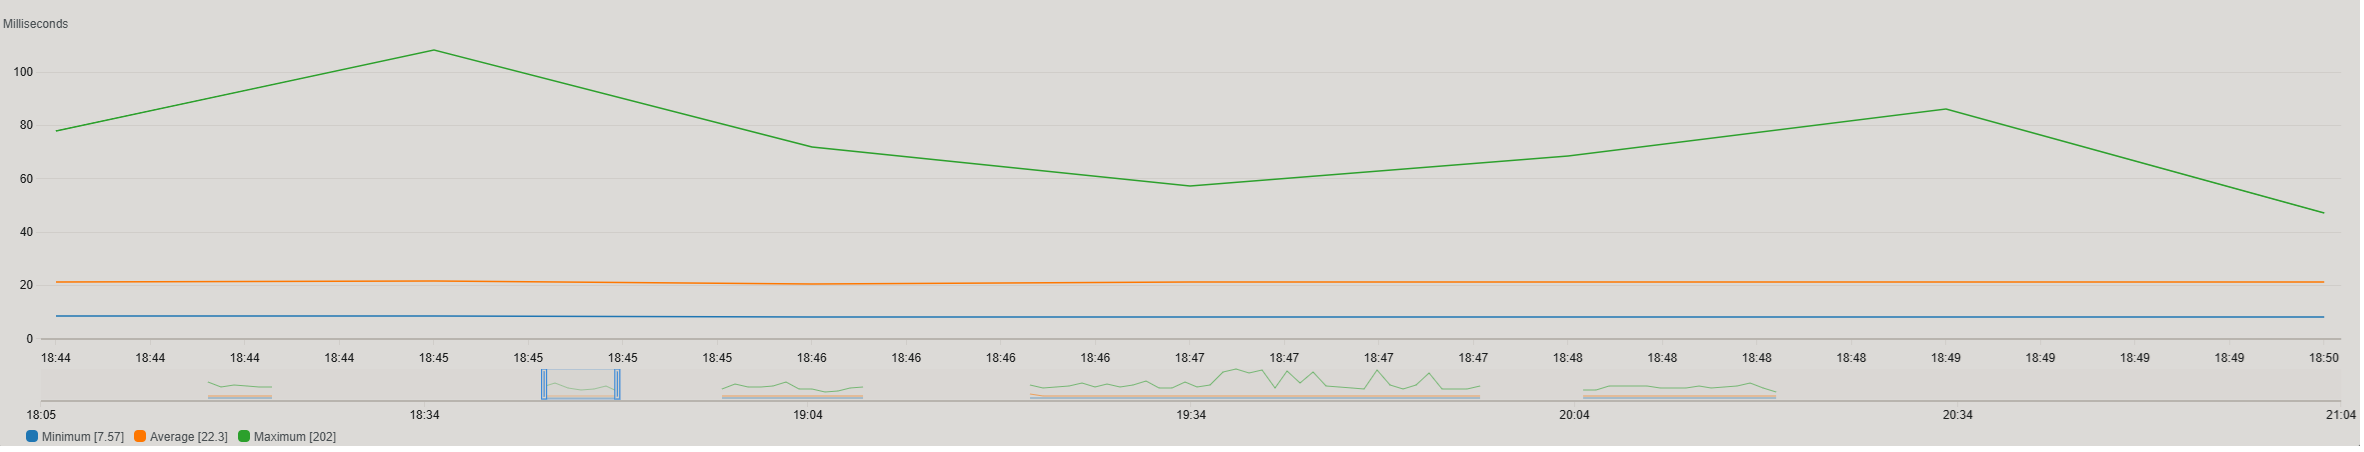
\includegraphics[width=.48\linewidth]{"figures/lA - Duration.png"}\hfill
  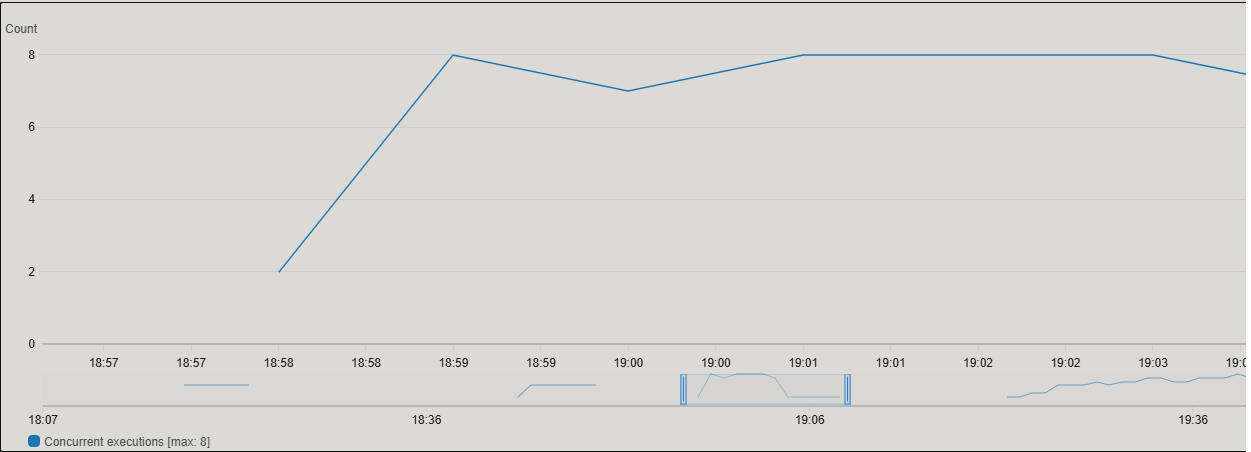
\includegraphics[width=.48\linewidth]{"figures/lA - ConcExecutions.png"}
  \caption{Light A --- Lambda Duration (left) and ConcurrentExecutions (right).}
\end{figure}

\paragraph{Heavy A (high-RPS bursty).}
Switching to near-zero client think time with 10 users converts A into a sustained high-throughput plateau. In Locust, the RPS rises sharply after WU. On the provider side, \emph{ConcurrentExecutions} plateaus near the Learner Lab ceiling (about 9--10), which is expected. \emph{Invocations} grow linearly over time during the steady phase, and \emph{Duration} maintains a tight band once the runtime is warm.

\begin{figure}[h!] \centering
  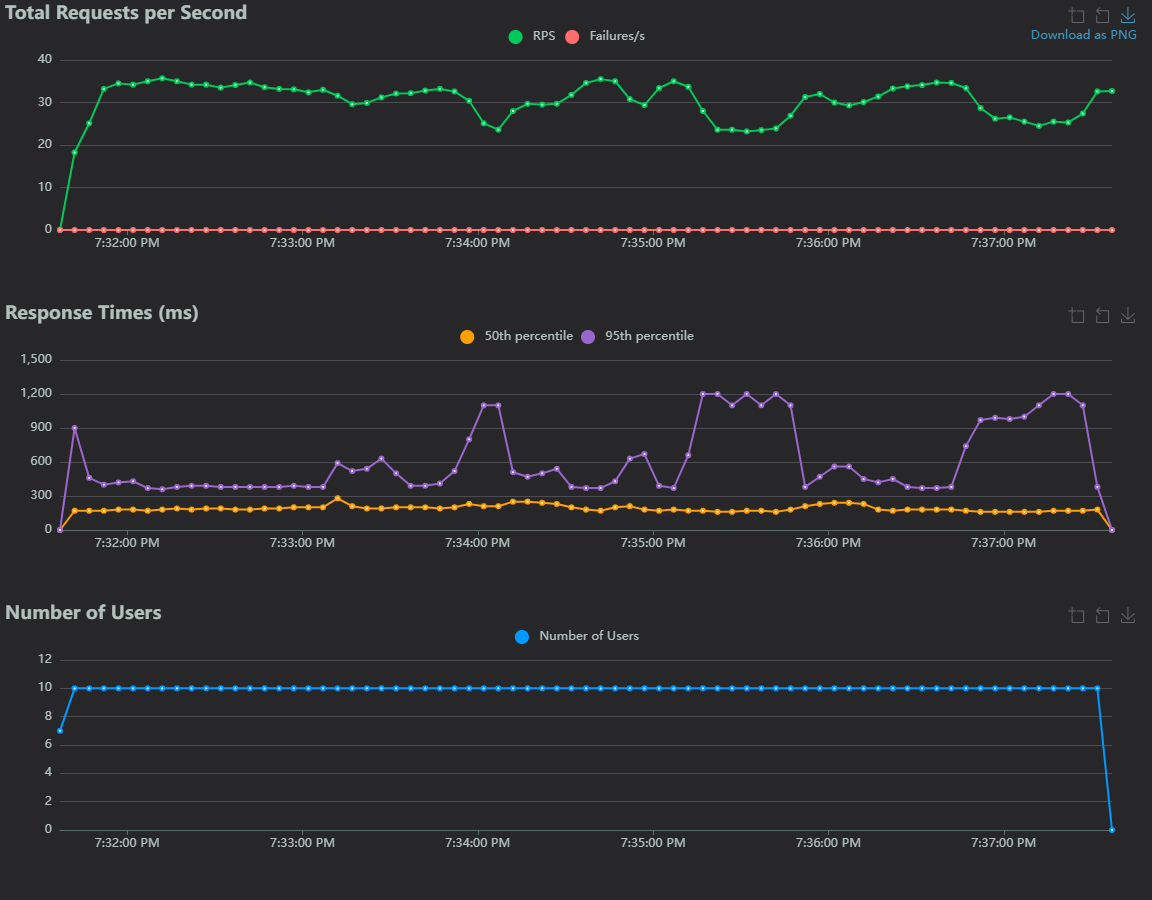
\includegraphics[width=\linewidth]{"figures/hA - Charts.png"}
  \caption{Heavy A --- Locust charts (RPS spike after WU; steady plateau).}
\end{figure}

\begin{figure}[h!] \centering
  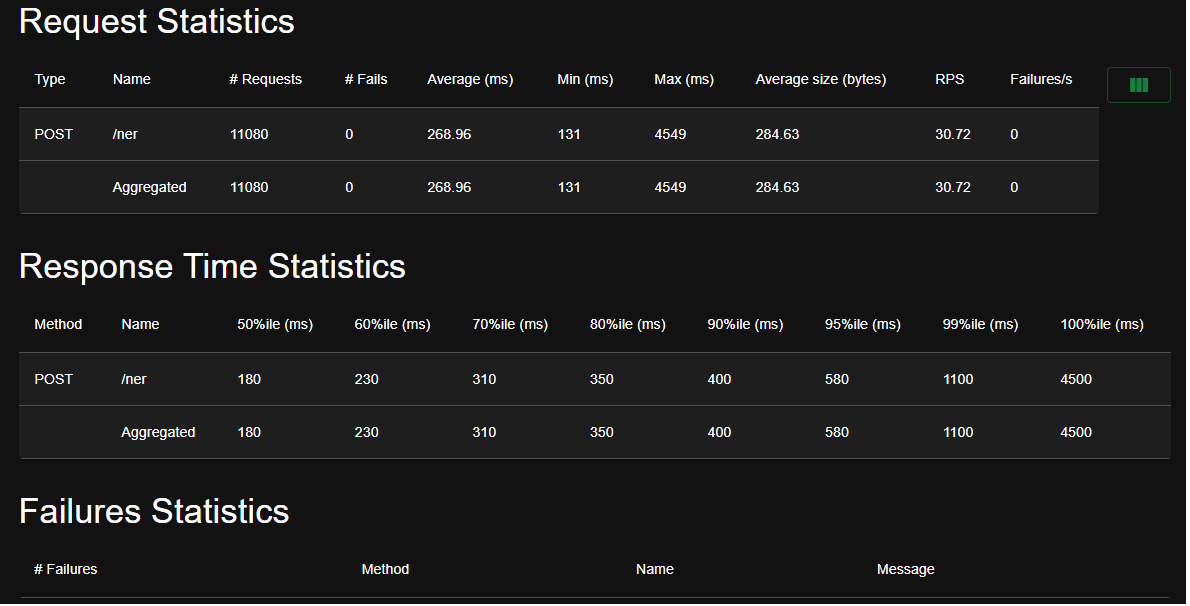
\includegraphics[width=\linewidth]{"figures/hA - Stats.png"}
  \caption{Heavy A --- Locust request statistics (p50/p95/p99, failures).}
\end{figure}

\begin{figure}[h!] \centering
  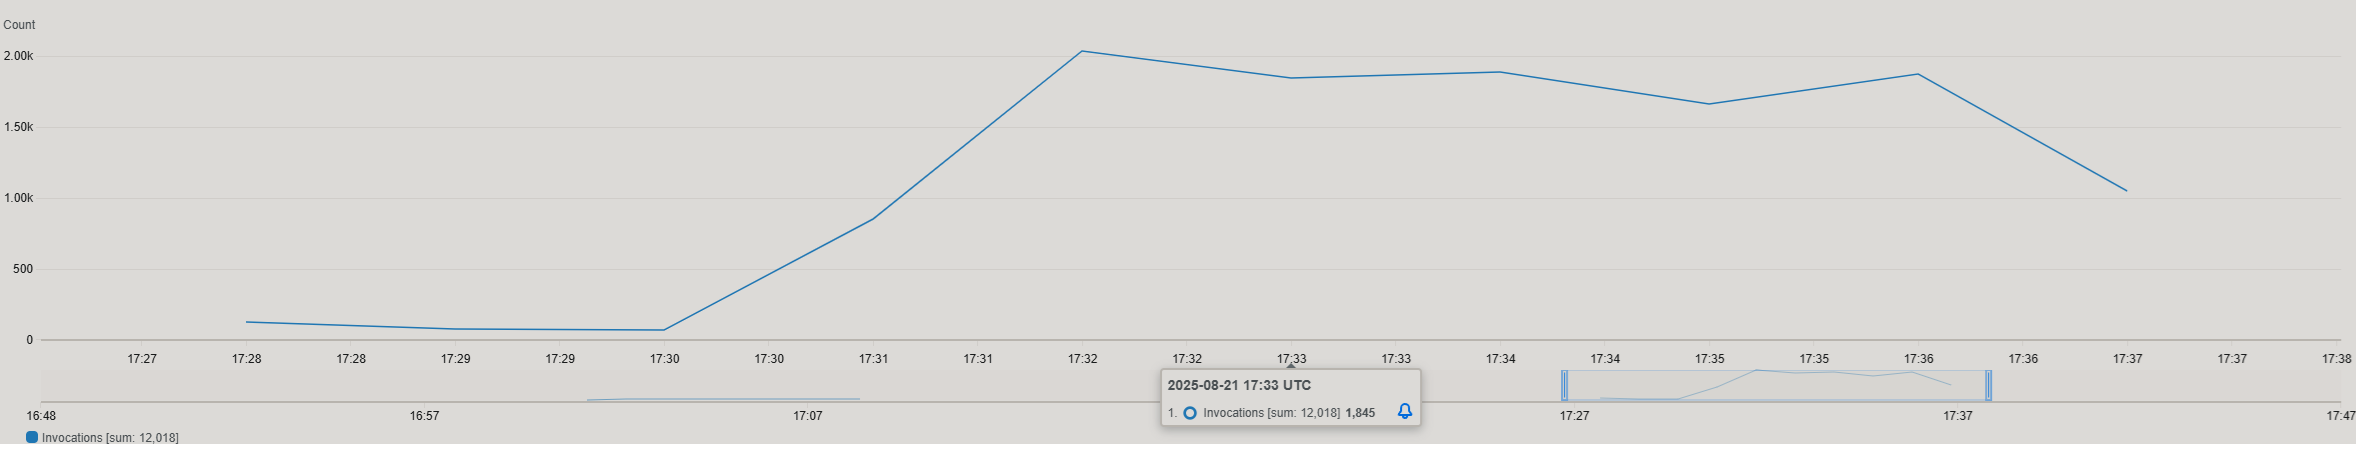
\includegraphics[width=.32\linewidth]{"figures/hA - Invocations.png"}\hfill
  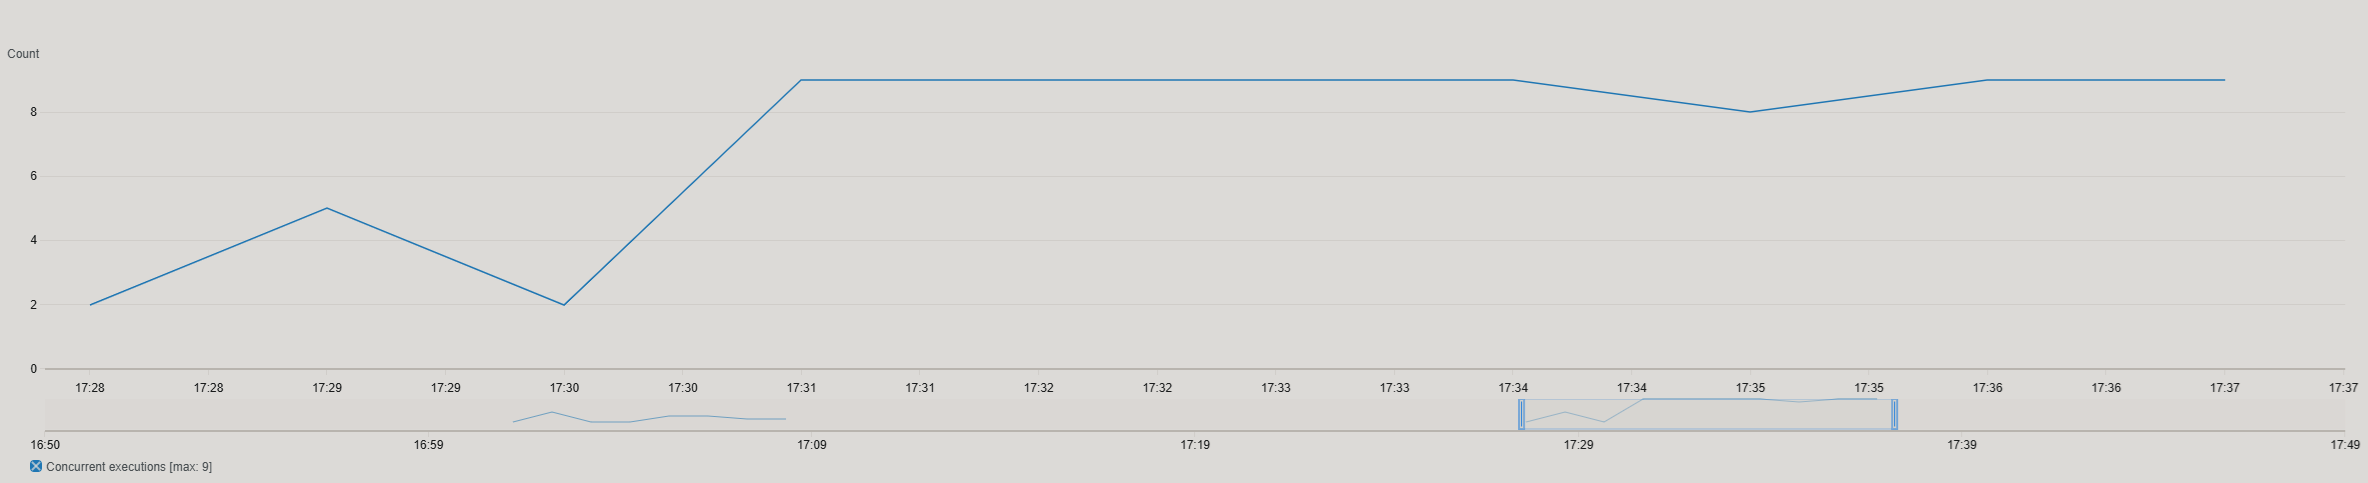
\includegraphics[width=.32\linewidth]{"figures/hA - ConcEx.png"}\hfill
  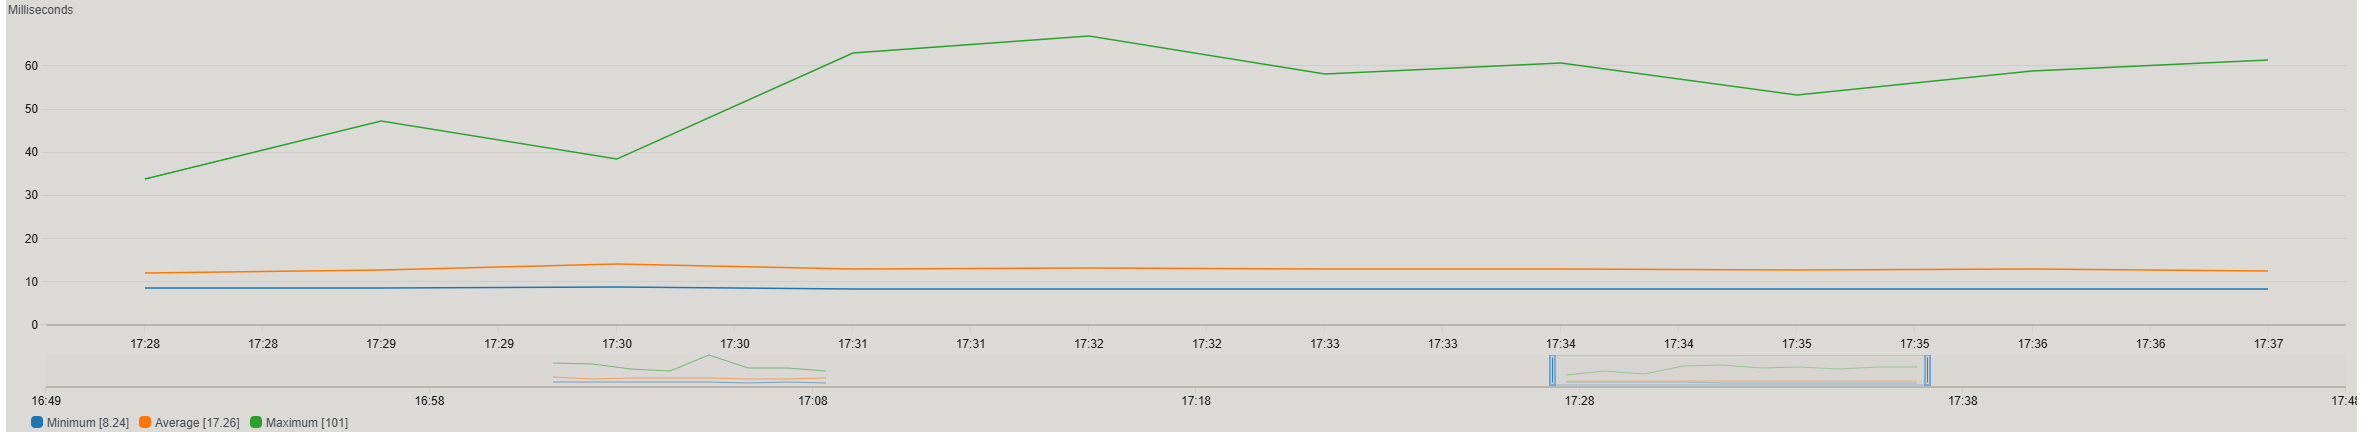
\includegraphics[width=.32\linewidth]{"figures/hA - Durations.png"}
  \caption{Heavy A --- Lambda Invocations (left), ConcurrentExecutions (middle), Duration (right).}
\end{figure}

\subsection{Scenario B (Ramp $\rightarrow$ Steady $\rightarrow$ Ramp-down)}\label{subsec:resB}

\paragraph{Light B (baseline shape).}
The Locust charts show the stair-step RU, a clear steady plateau, and a controlled RD. Latency percentiles track this shape with mild variations, as expected under moderate load. Lambda \emph{Invocations} and \emph{ConcurrentExecutions} rise predictably during RU and flatten during the steady window.

\begin{figure}[h!] \centering
  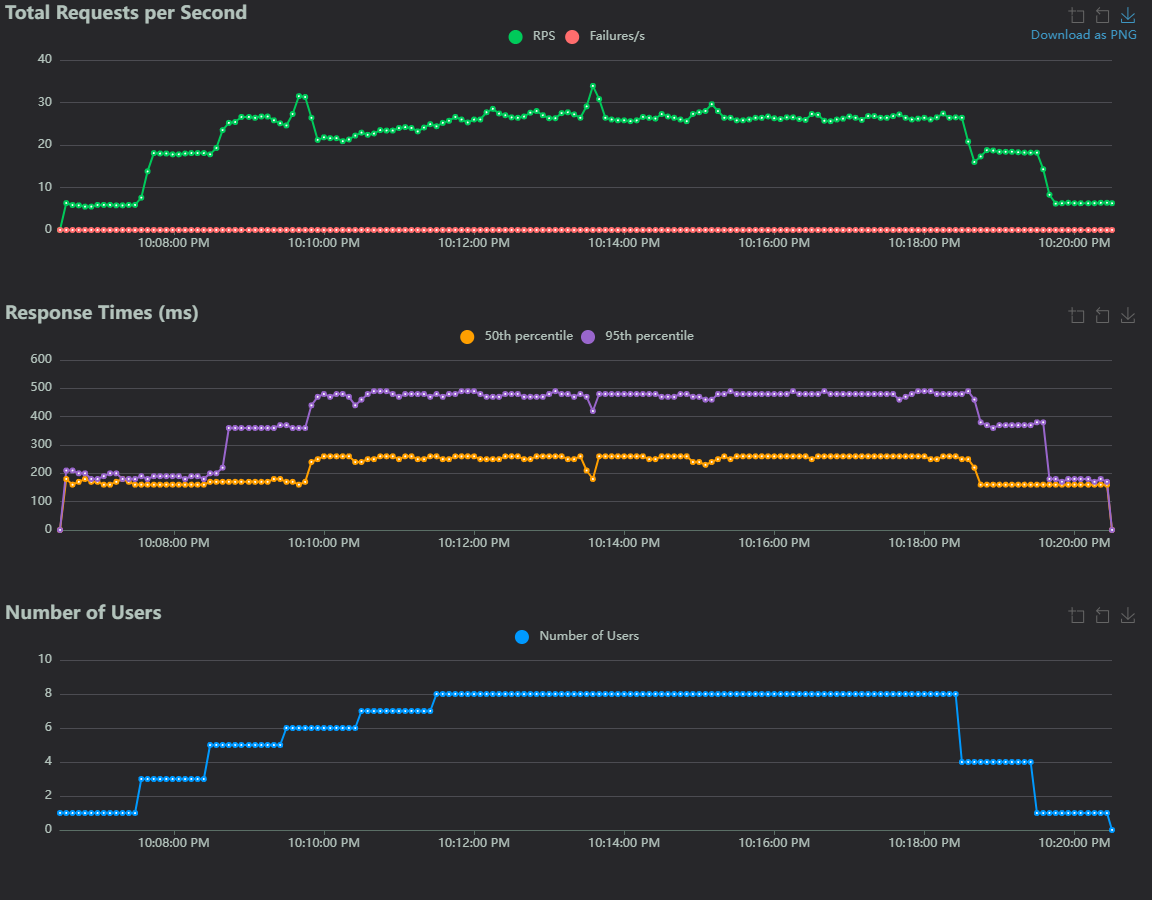
\includegraphics[width=\linewidth]{"figures/lB - Charts.png"}
  \caption{Light B --- Locust charts (ramp, steady plateau, ramp-down).}
\end{figure}

\begin{figure}[h!] \centering
  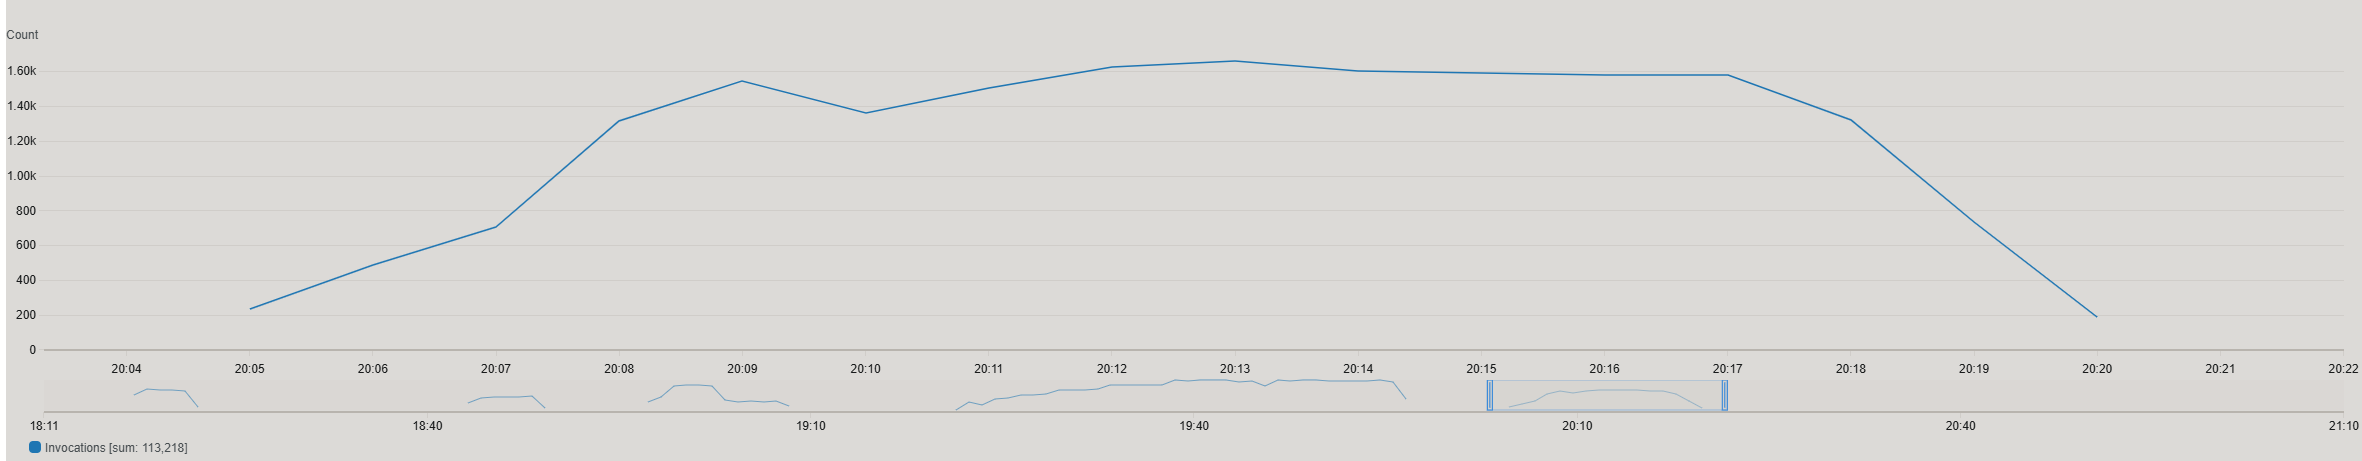
\includegraphics[width=.32\linewidth]{"figures/lB - Invocations.png"}\hfill
  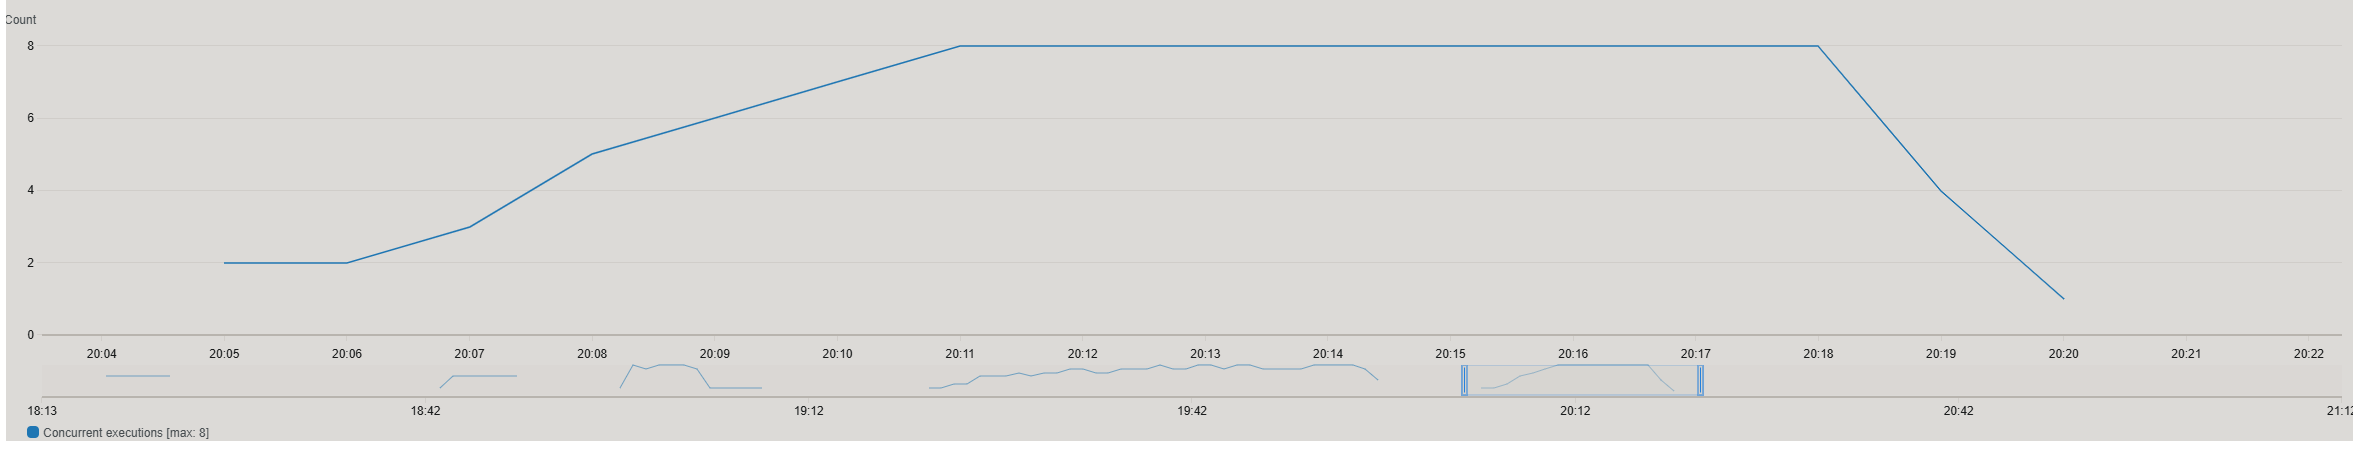
\includegraphics[width=.32\linewidth]{"figures/lB - ConcEx.png"}\hfill
  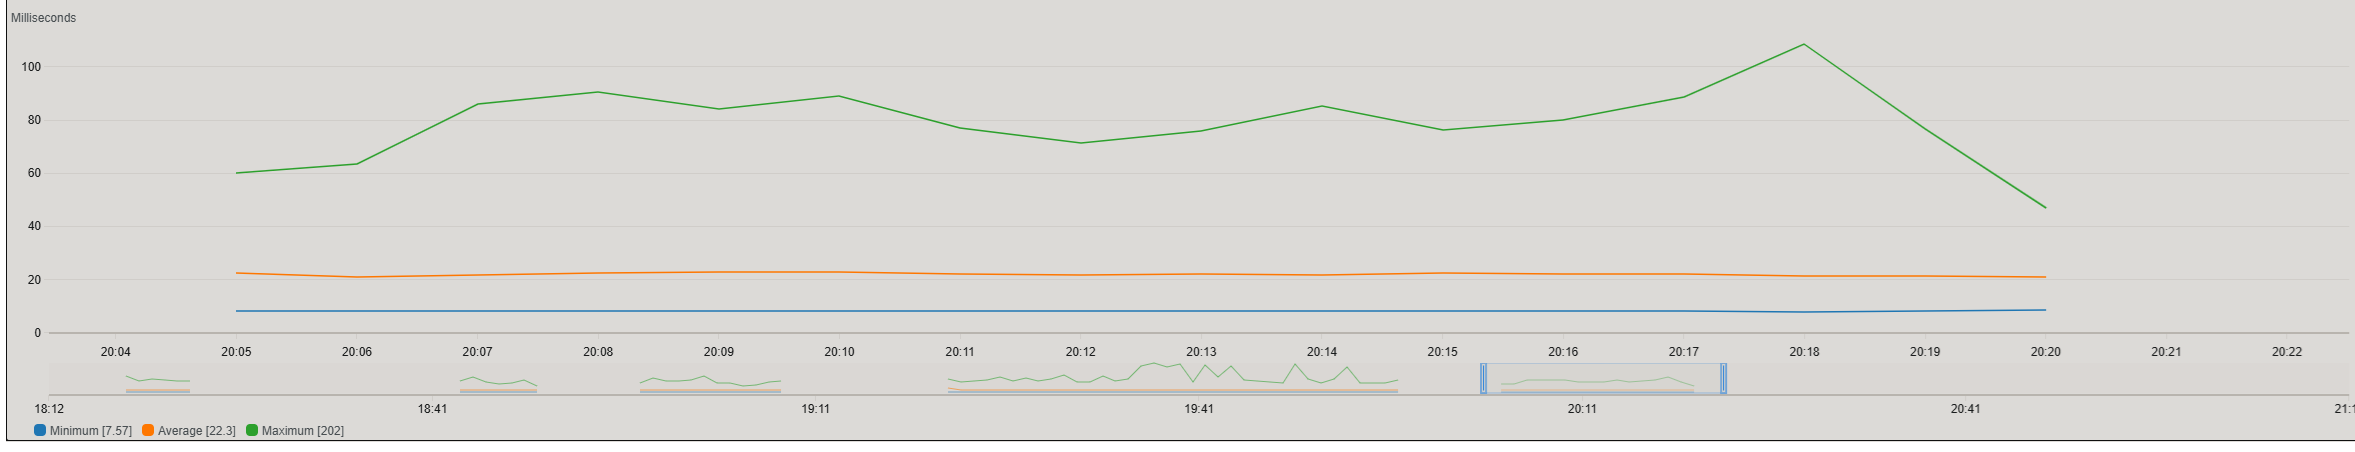
\includegraphics[width=.32\linewidth]{"figures/lB - Duration.png"}
  \caption{Light B --- Lambda Invocations, ConcurrentExecutions, Duration.}
\end{figure}

\paragraph{Heavy B @ \SI{1024}{MB} (high-RPS ramp/steady).}
With near-zero think time and 10 users, Heavy B reaches a higher RPS plateau than Light B while preserving the RU/S/RD structure. Locust statistics show tightened latency percentiles during the steady phase, indicating that the function remains comfortably within its latency budget under sustained load. Lambda \emph{ConcurrentExecutions} plateaus close to the concurrency limit; \emph{Duration} stabilizes to a narrow band after RU; \emph{Invocations} show the expected linear accumulation over the steady window.

\begin{figure}[h!] \centering
  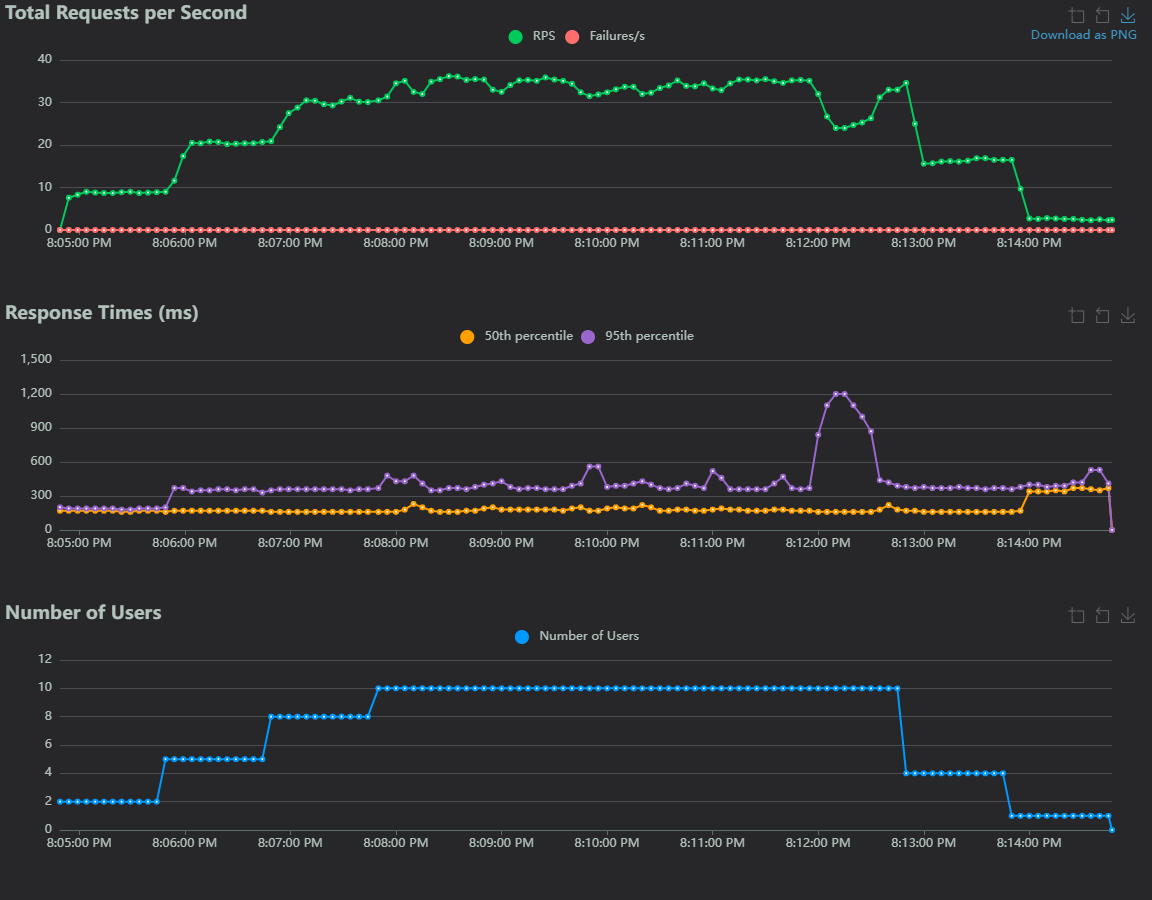
\includegraphics[width=\linewidth]{"figures/hB - Charts.png"}
  \caption{Heavy B (1024 MB) --- Locust charts (higher RPS plateau vs Light).}
\end{figure}

\begin{figure}[h!] \centering
  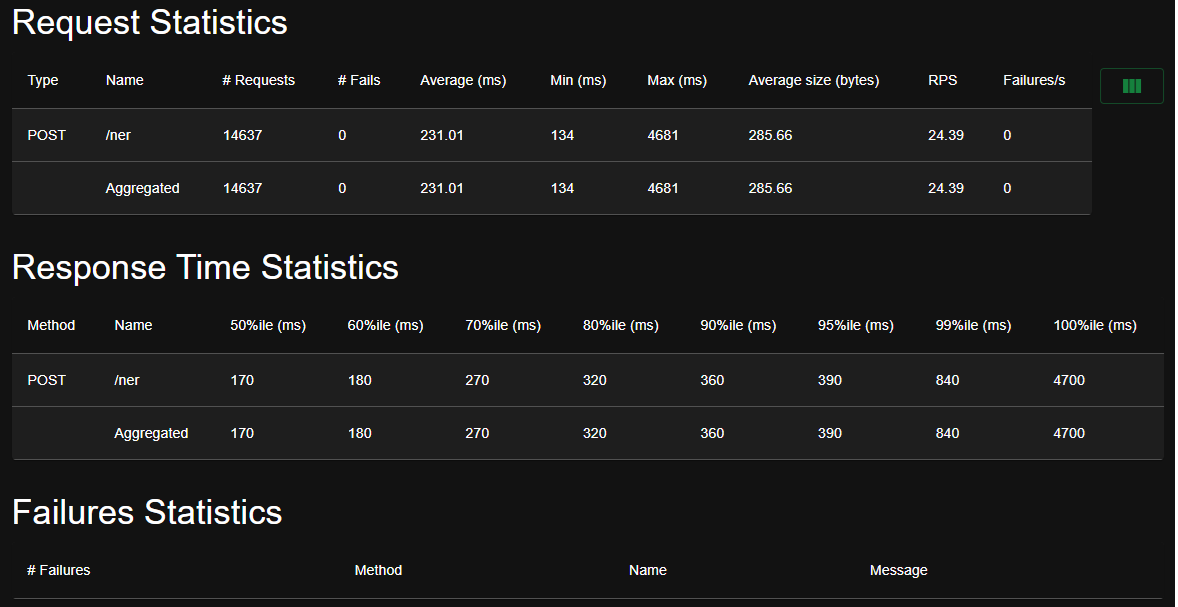
\includegraphics[width=\linewidth]{"figures/hB - Stats.png"}
  \caption{Heavy B (1024 MB) --- Locust request statistics.}
\end{figure}

\begin{figure}[h!] \centering
  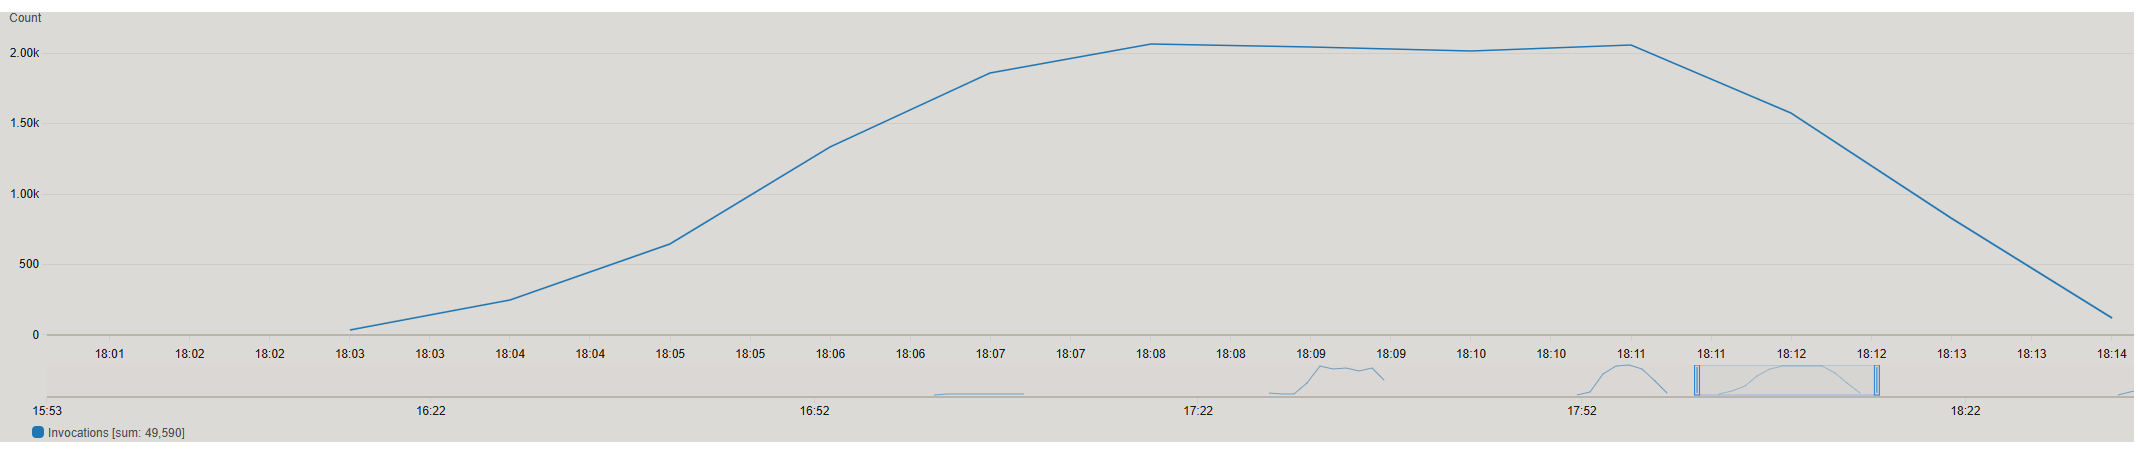
\includegraphics[width=.32\linewidth]{"figures/hB - Invocations.png"}\hfill
  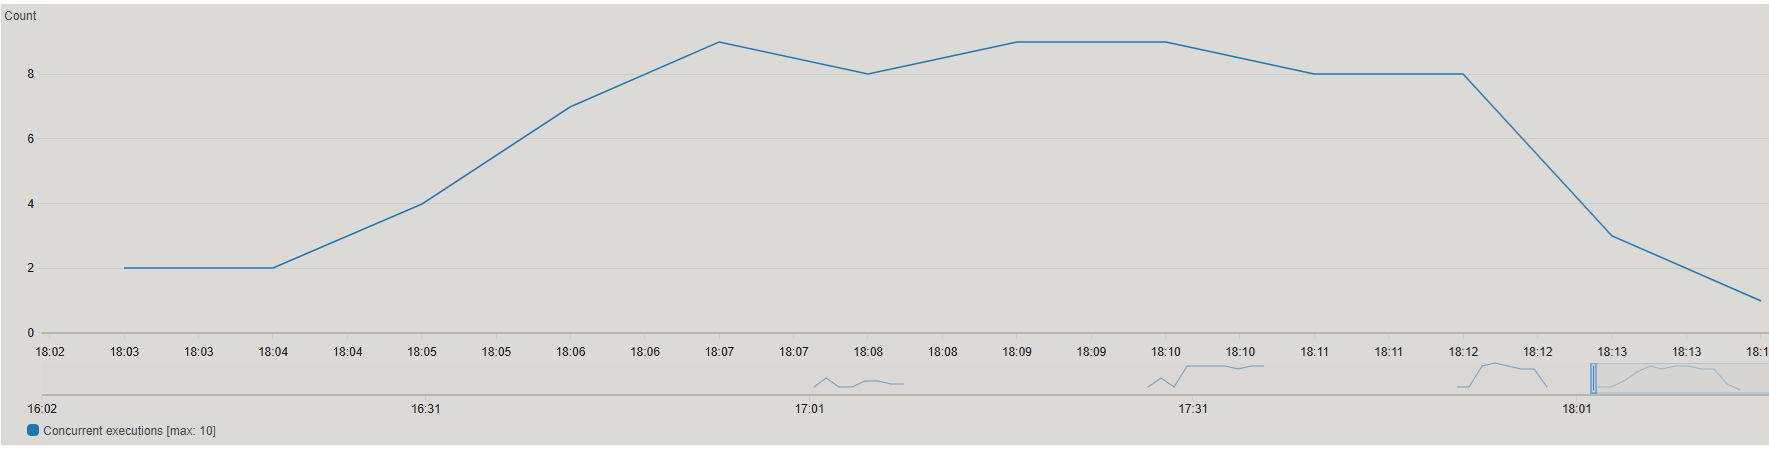
\includegraphics[width=.32\linewidth]{"figures/hB - ConcEx.png"}\hfill
  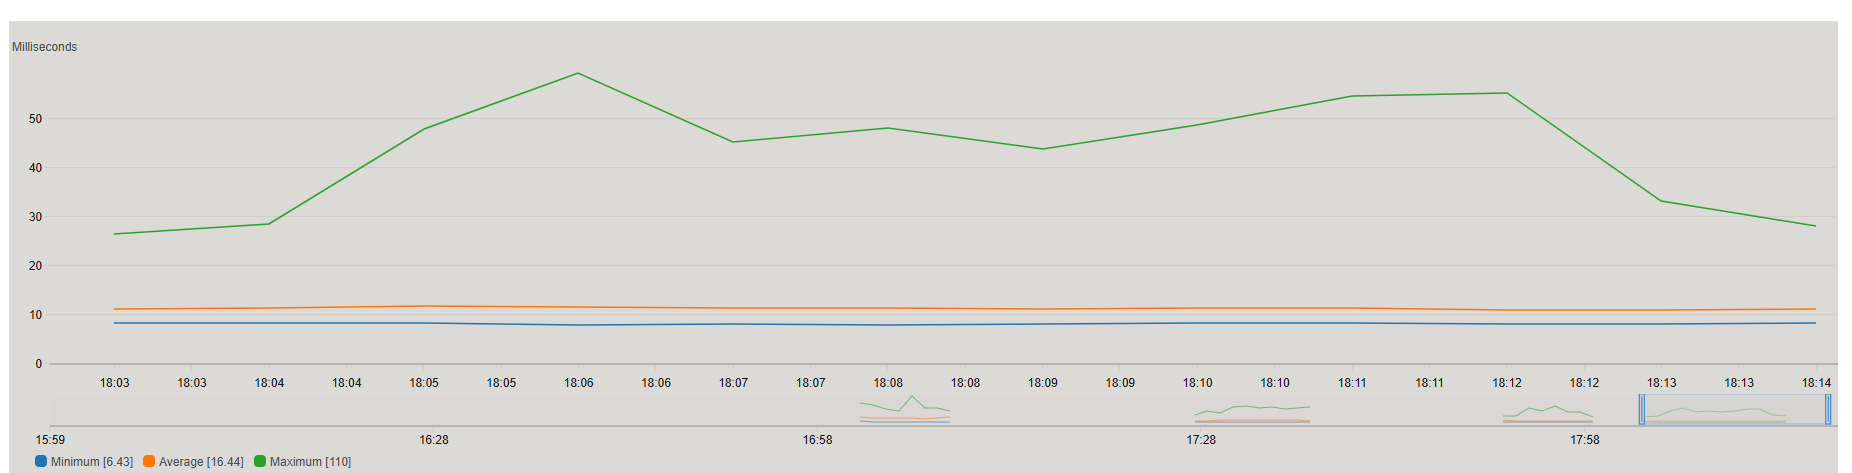
\includegraphics[width=.32\linewidth]{"figures/hB - Duration.png"}
  \caption{Heavy B (1024 MB) --- Lambda Invocations, ConcurrentExecutions, Duration.}
\end{figure}

\paragraph{Vertical scaling: Heavy B @ \SI{512}{MB} vs @ \SI{1024}{MB}.}
We re-executed the identical Heavy B shape at \SI{512}{MB} (\texttt{hBl-*}) to isolate the impact of memory. The comparison is clearest during the steady window:
\begin{itemize}
  \item \textbf{Latency effect:} The \SI{1024}{MB} configuration exhibits lower and tighter p95/p99 latency bands than \SI{512}{MB}, consistent with the expectation that more memory (and CPU share) shortens inference time. This is visible in the Lambda \emph{Duration} time series and in the Locust percentiles.
  \item \textbf{Throughput effect:} Because the account-level concurrency limit remains the same, higher memory primarily improves \emph{per-invocation} speed rather than concurrency. As a result, the steady-state RPS at \SI{1024}{MB} is higher than at \SI{512}{MB} for the same user pacing, and the system reaches the plateau faster during RU.
  \item \textbf{Stability:} Both memory settings remain stable during the steady window; no persistent spikes or oscillations are evident. If any brief spikes are present, they align with RU steps and do not persist in S.
\end{itemize}

\begin{figure}[h!] \centering
  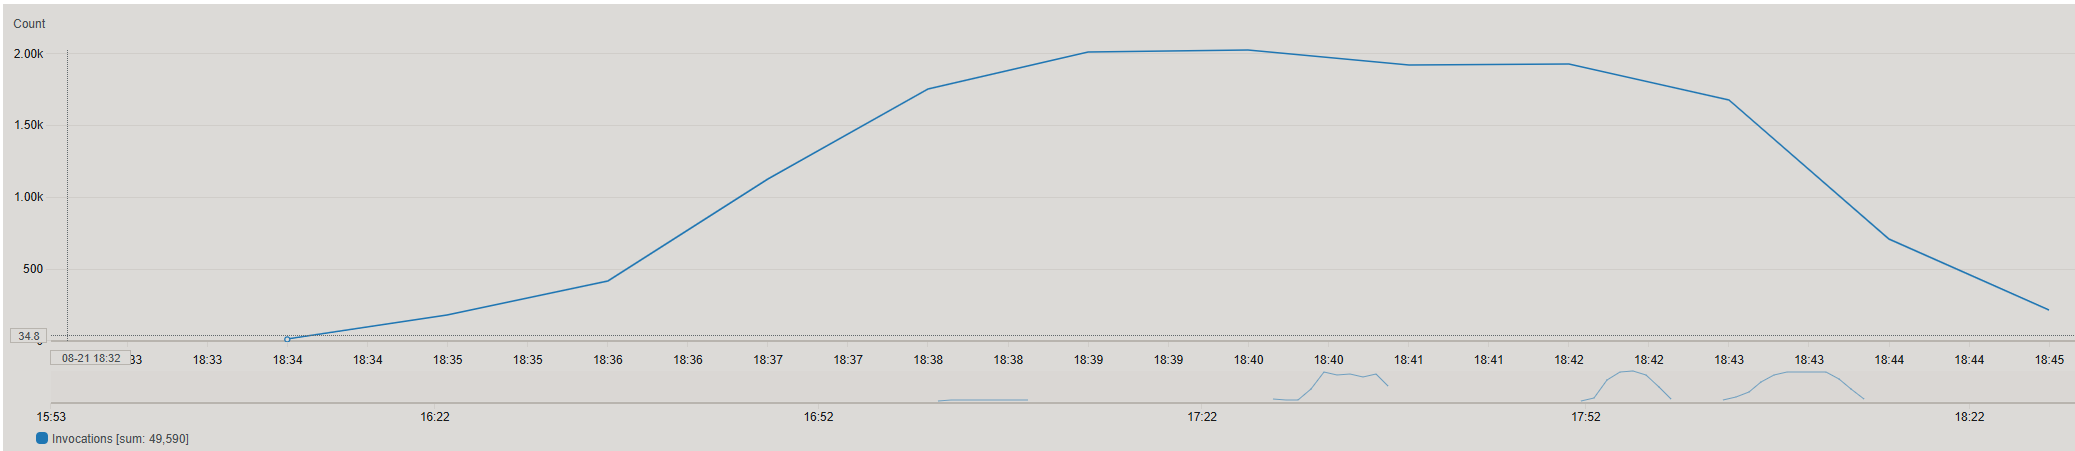
\includegraphics[width=.32\linewidth]{"figures/hBl - Invocations.png"}\hfill
  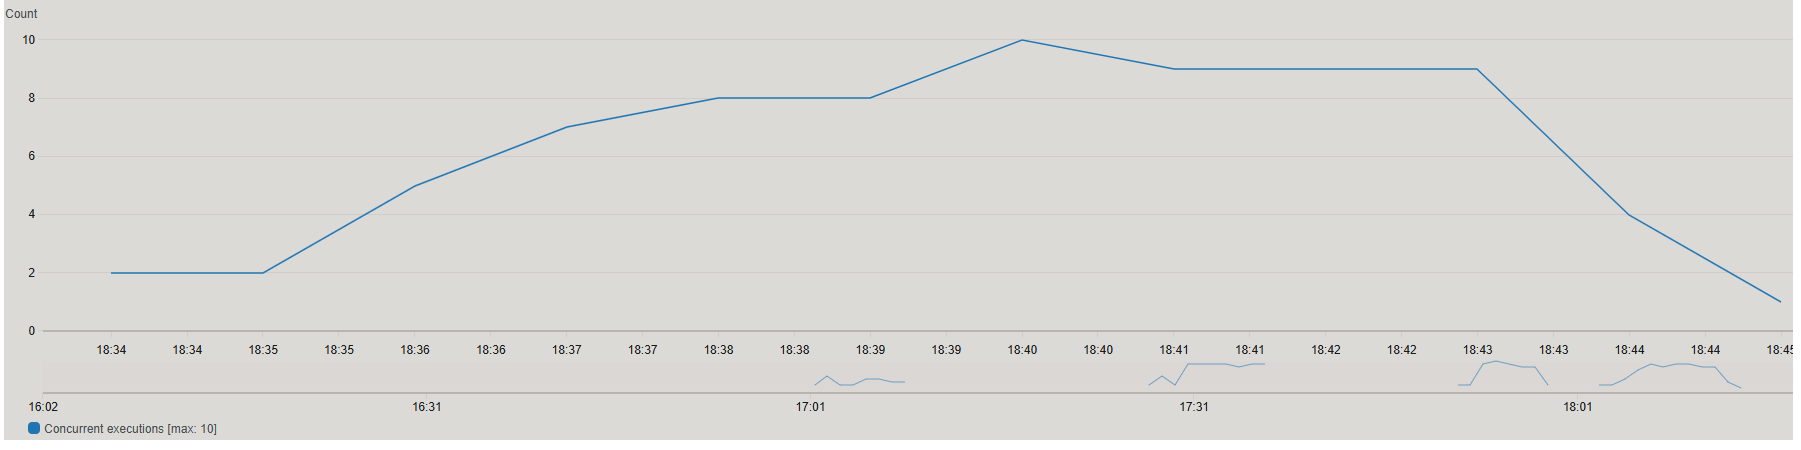
\includegraphics[width=.32\linewidth]{"figures/hBl - ConcEx.png"}\hfill
  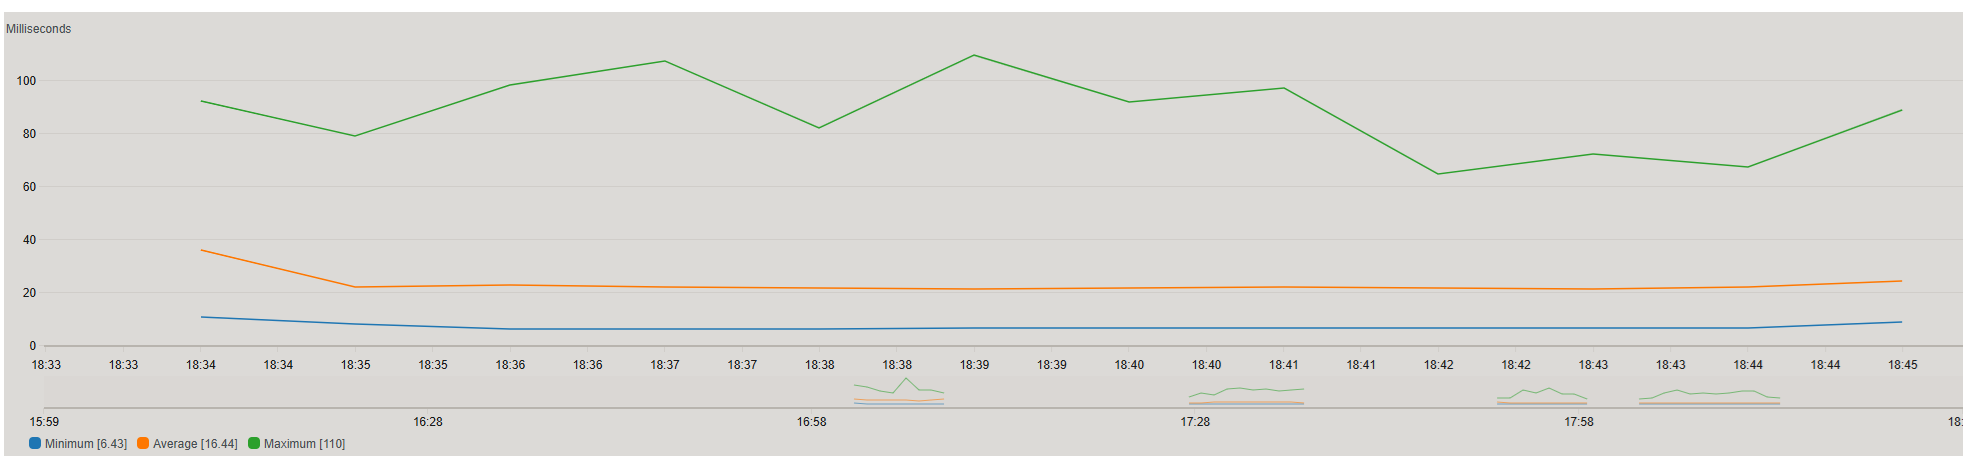
\includegraphics[width=.32\linewidth]{"figures/hBl - Duration.png"}
  \caption{Heavy B (512 MB) --- Lambda Invocations, ConcurrentExecutions, Duration.}
\end{figure}

\begin{figure}[h!] \centering
  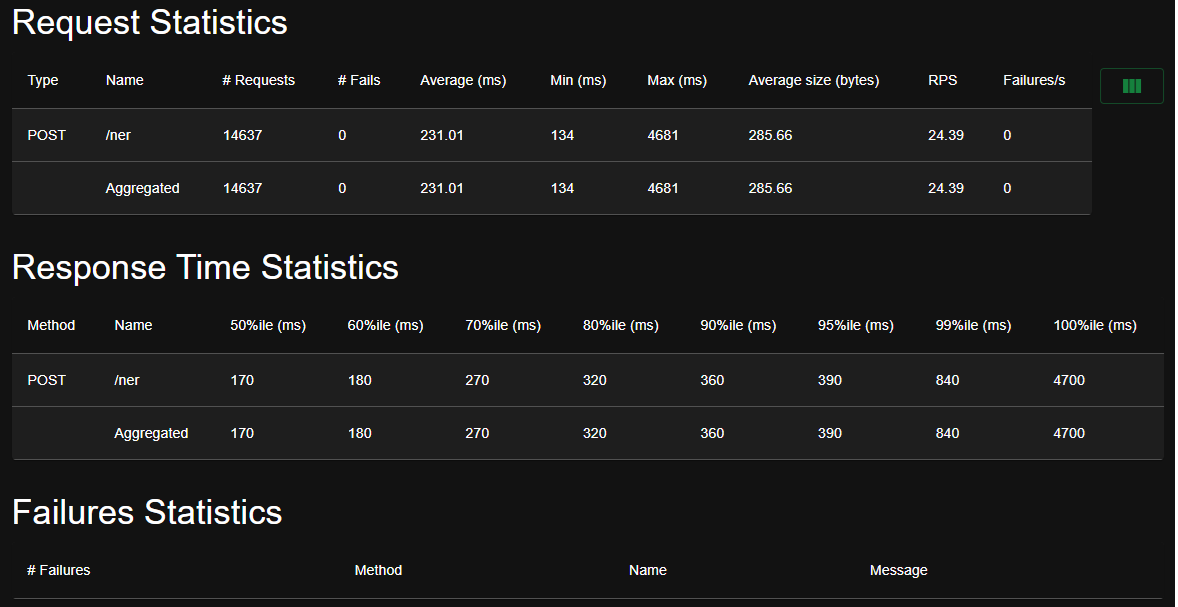
\includegraphics[width=.49\linewidth]{"figures/hB - Stats.png"}\hfill
  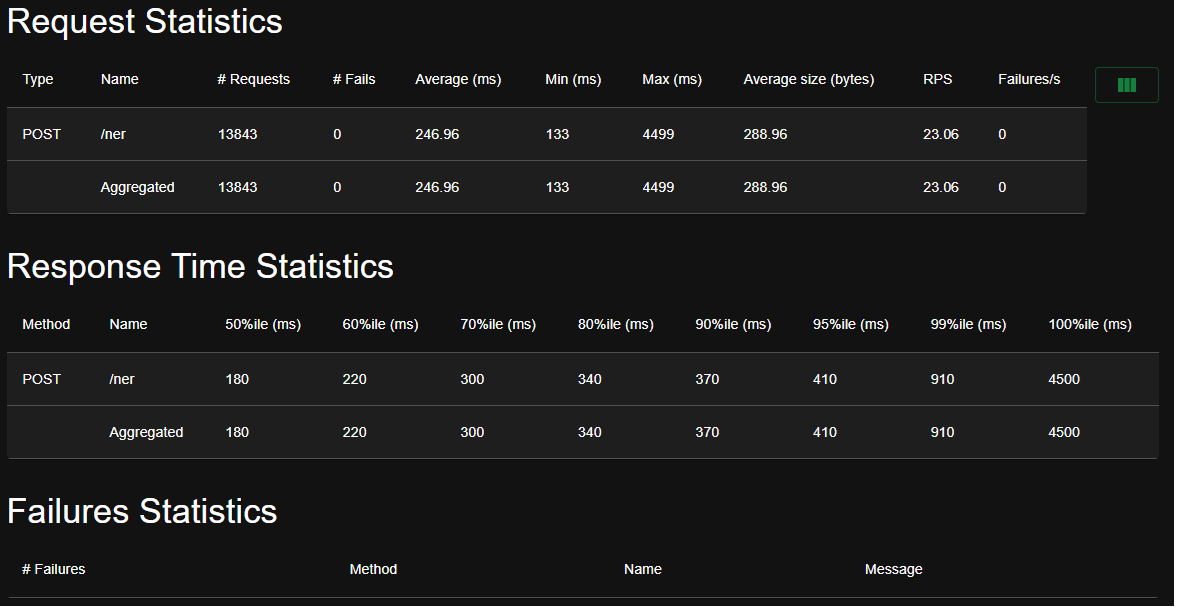
\includegraphics[width=.49\linewidth]{"figures/hBl - Stats.png"}
  \caption{Heavy B --- Locust request statistics: 1024 MB (left) vs 512 MB (right).}
\end{figure}

\subsection{Scenario C (Spike)}\label{subsec:resC}

\paragraph{Light C (moderate spike).}
After a short pre-spike, the user count jumps to the steady segment and then drops. Locust shows the expected RPS surge and recovery, with latency percentiles temporarily stretching at the spike boundary and then stabilizing. Lambda \emph{ConcurrentExecutions} mirrors the spike profile; \emph{Invocations} reflect the burst in requests; \emph{Duration} remains in a narrow band during the steady segment.

\begin{figure}[h!] \centering
  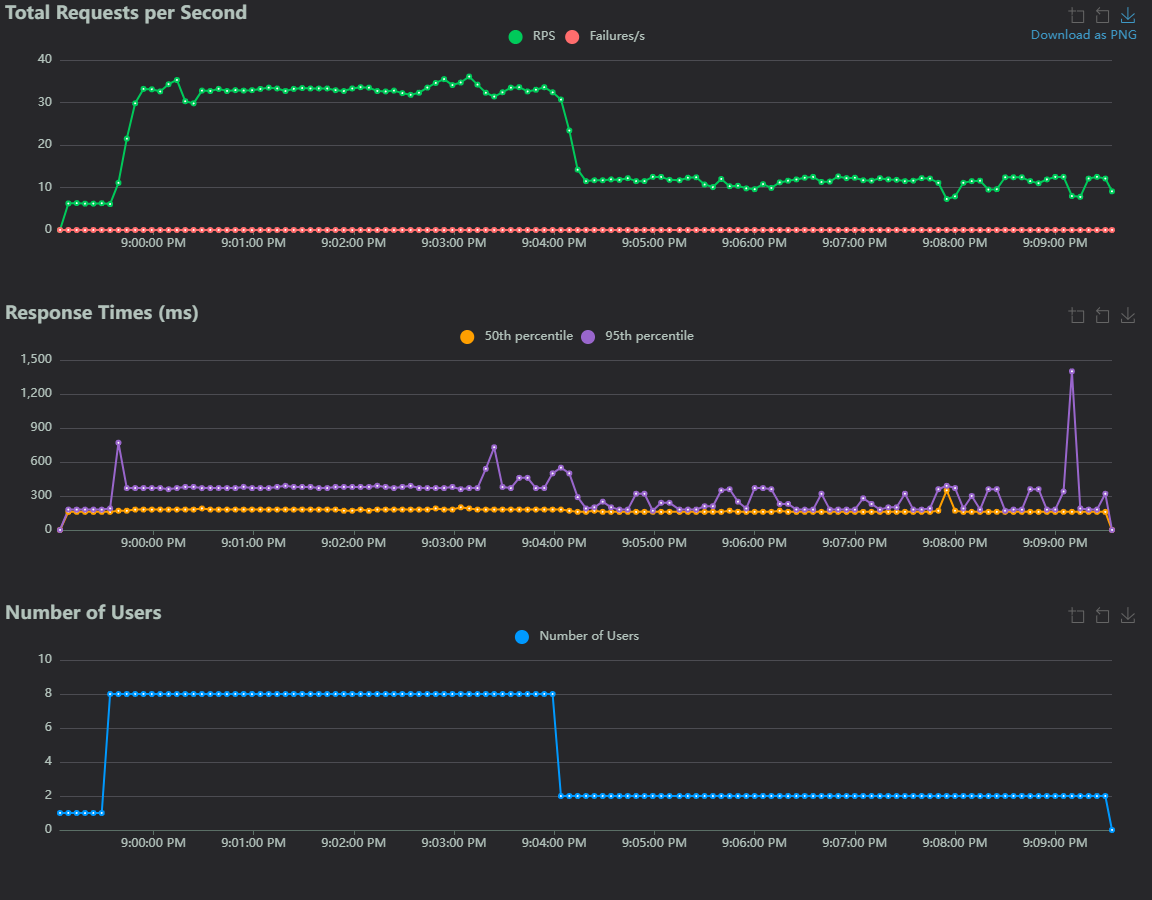
\includegraphics[width=\linewidth]{"figures/lC - Charts.png"}
  \caption{Light C --- Locust charts (spike).}
\end{figure}

\begin{figure}[h!] \centering
  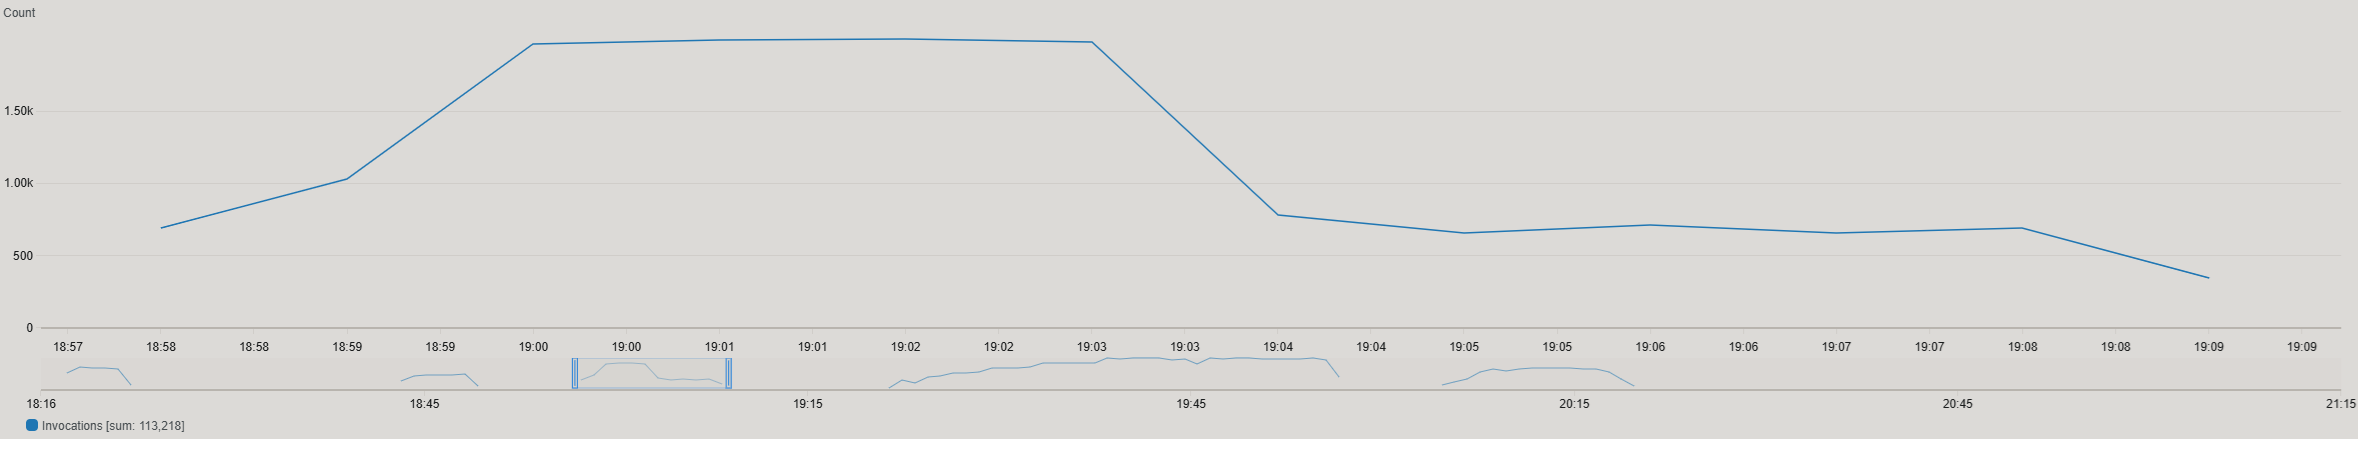
\includegraphics[width=.32\linewidth]{"figures/lC - Invocations.png"}\hfill
  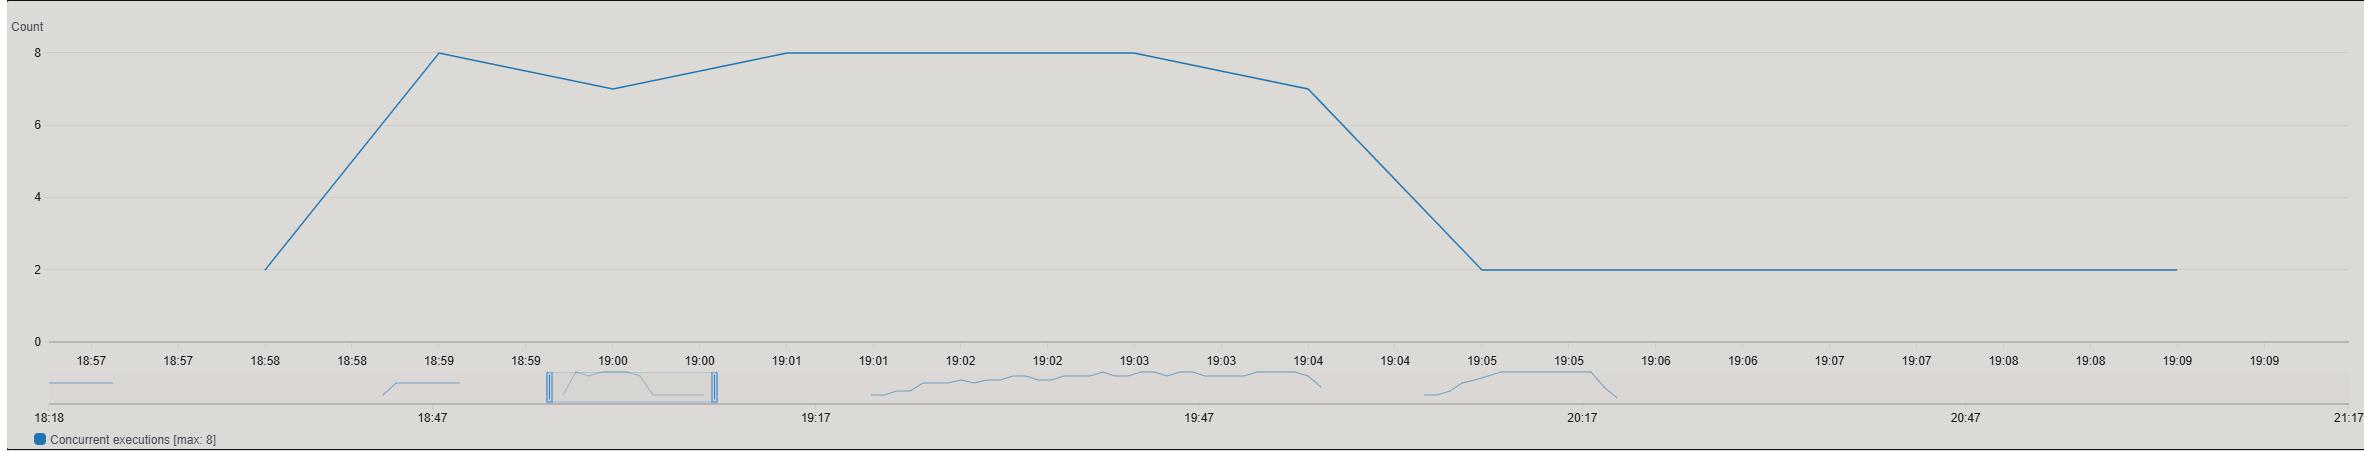
\includegraphics[width=.32\linewidth]{"figures/lC - ConcEx.png"}\hfill
  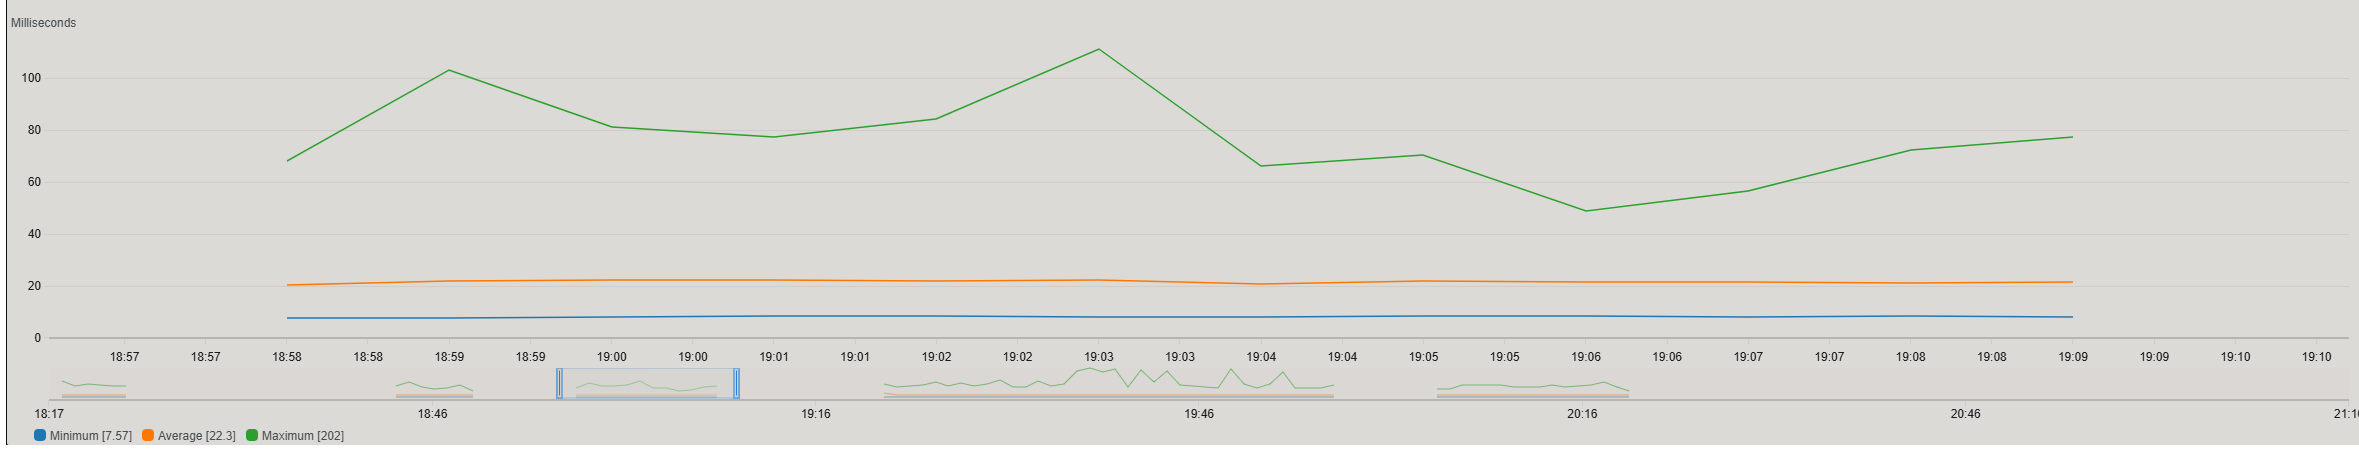
\includegraphics[width=.32\linewidth]{"figures/lC - Duration.png"}
  \caption{Light C --- Lambda Invocations, ConcurrentExecutions, Duration.}
\end{figure}

\paragraph{Heavy C (high-intensity spike @ \SI{1024}{MB}).}
With near-zero think time and 10 users, the spike immediately drives the system to the concurrency limit. Locust shows a sharp RPS jump with stable percentiles in the middle of the spike; Lambda confirms the concurrency plateau and a consistent \emph{Duration} band. The swift stabilization after the spike indicates that the cold-start penalty has been amortized during WU and the system sustains the intensity without degradation.

\begin{figure}[h!] \centering
  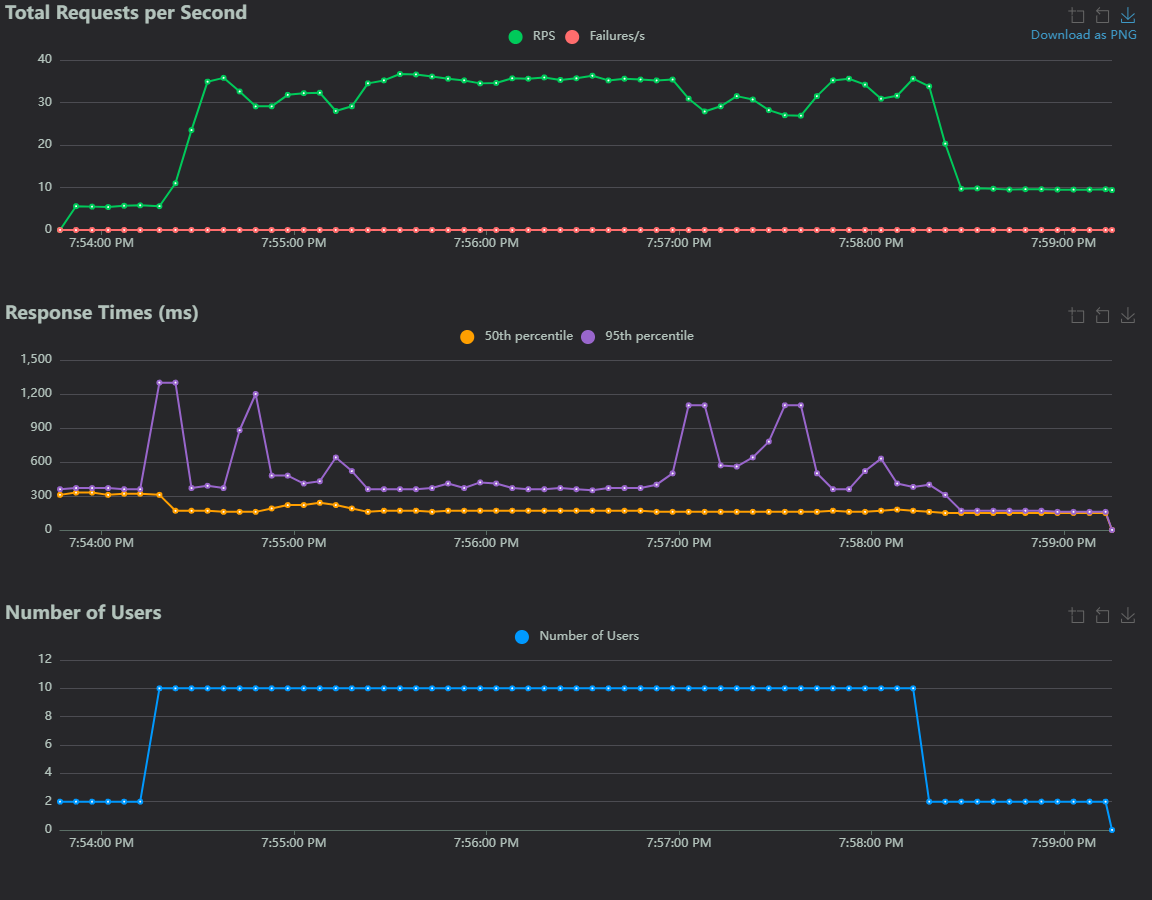
\includegraphics[width=\linewidth]{"figures/hC - Charts.png"}
  \caption{Heavy C --- Locust charts (high-intensity spike).}
\end{figure}

\begin{figure}[h!] \centering
  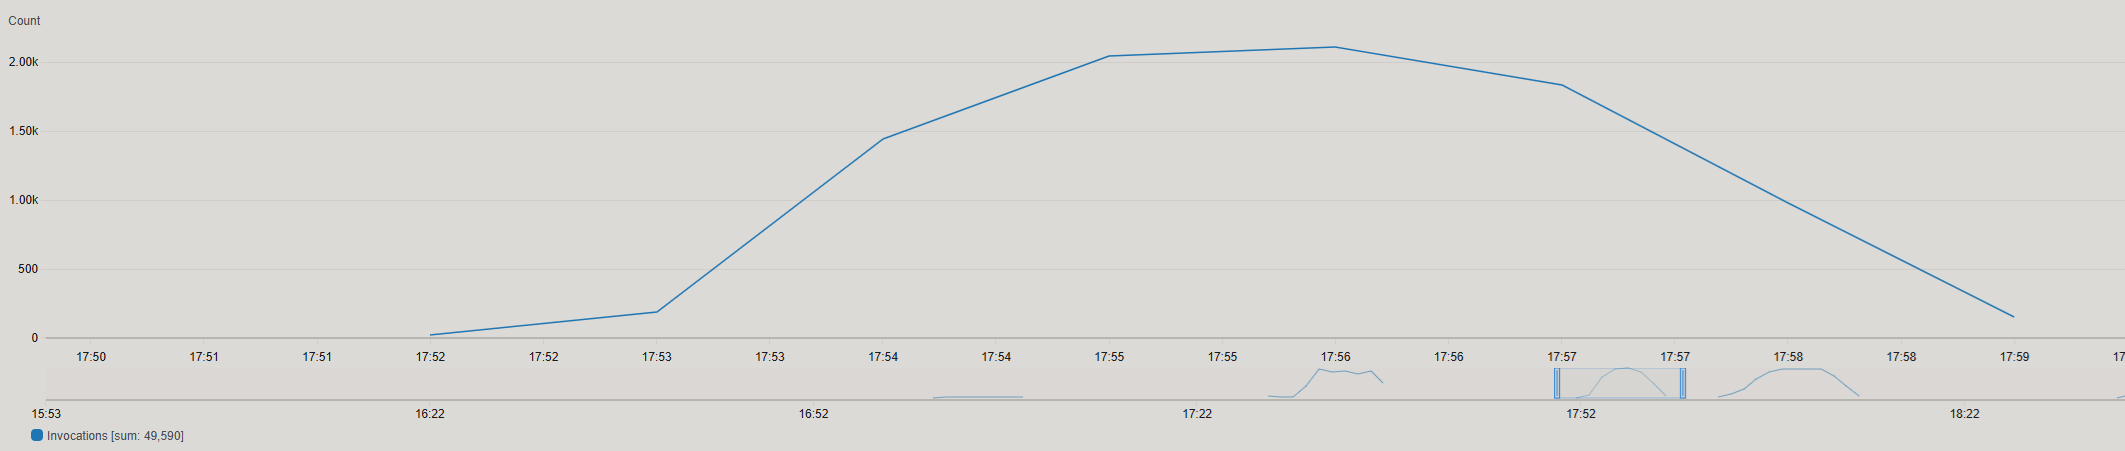
\includegraphics[width=.32\linewidth]{"figures/hC - Invocations.png"}\hfill
  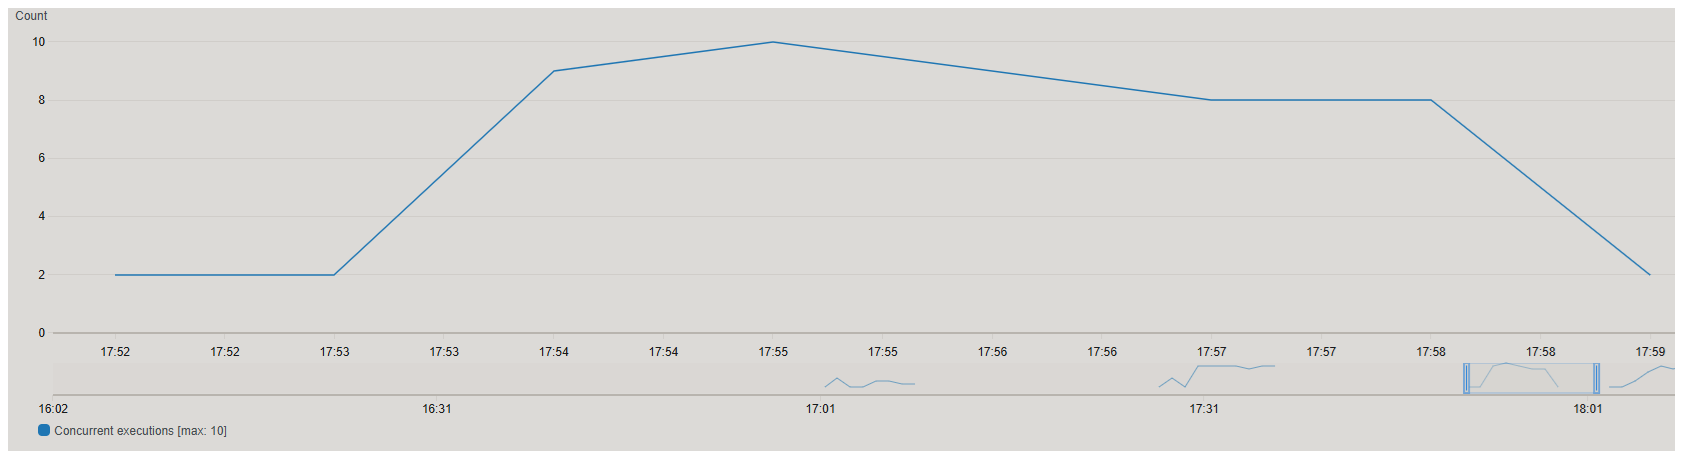
\includegraphics[width=.32\linewidth]{"figures/hC - ConcEx.png"}\hfill
  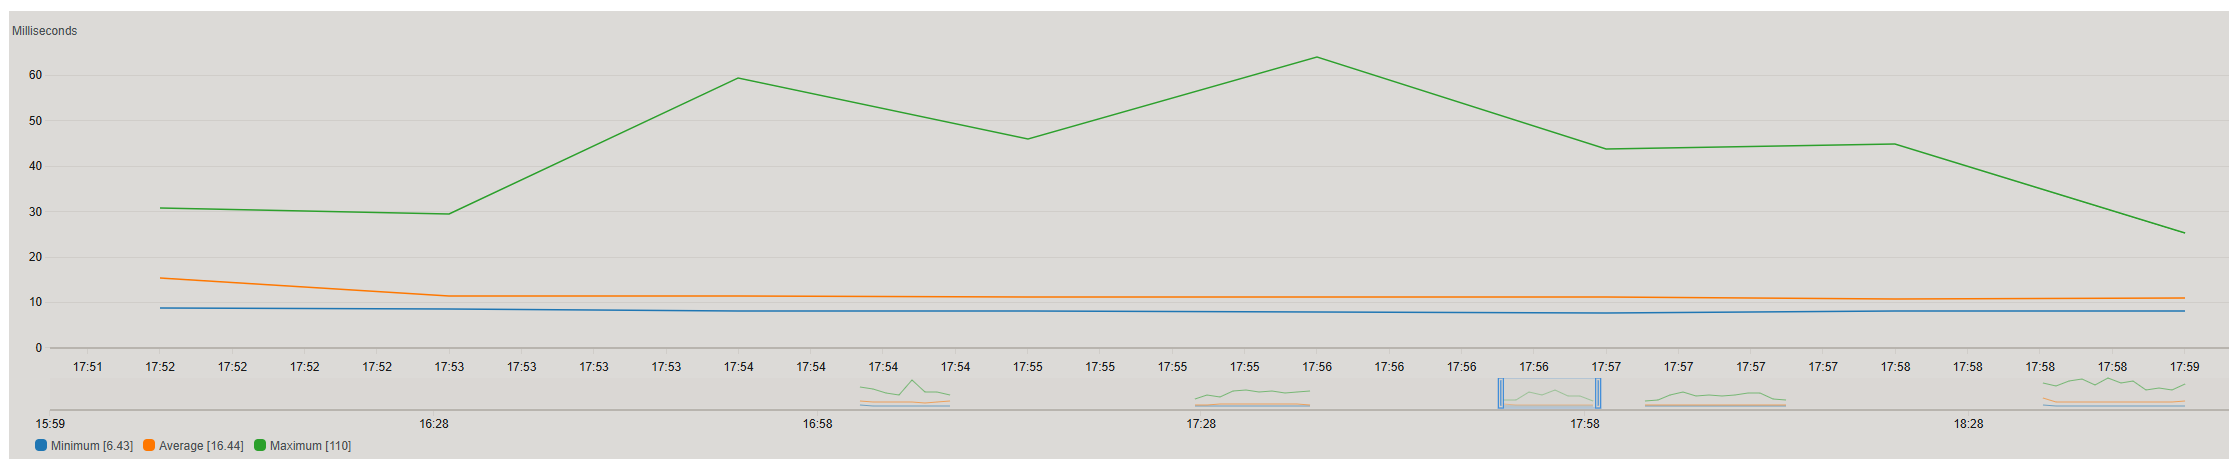
\includegraphics[width=.32\linewidth]{"figures/hC - Duration.png"}
  \caption{Heavy C --- Lambda Invocations, ConcurrentExecutions, Duration.}
\end{figure}

\paragraph{Very Heavy A (``hhA''): WU 30\,s + 180\,s window, 40 users, low per-user pacing.}
We executed an additional, more aggressive variant of scenario~A to probe headroom once concurrency is raised on the client side. The shape preserves the bursty pattern (rapid climb after WU, then a long steady plateau), but we increased the active users to 40 and kept per-user think times very small to emphasize arrival rate.

Locust shows a clean rise to a sustained throughput of \(\sim\)60--70~RPS with zero failures throughout the steady window; p50/p95 latencies stabilize in the \(\sim\)0.64\,s / \(\sim\)0.73\,s range, respectively, after a short warm-up spike. The maximum latency over the whole run is a single outlier (\(\sim\)6.9\,s) during the transition, which does not persist in the steady state.

\begin{figure}[h!]\centering
  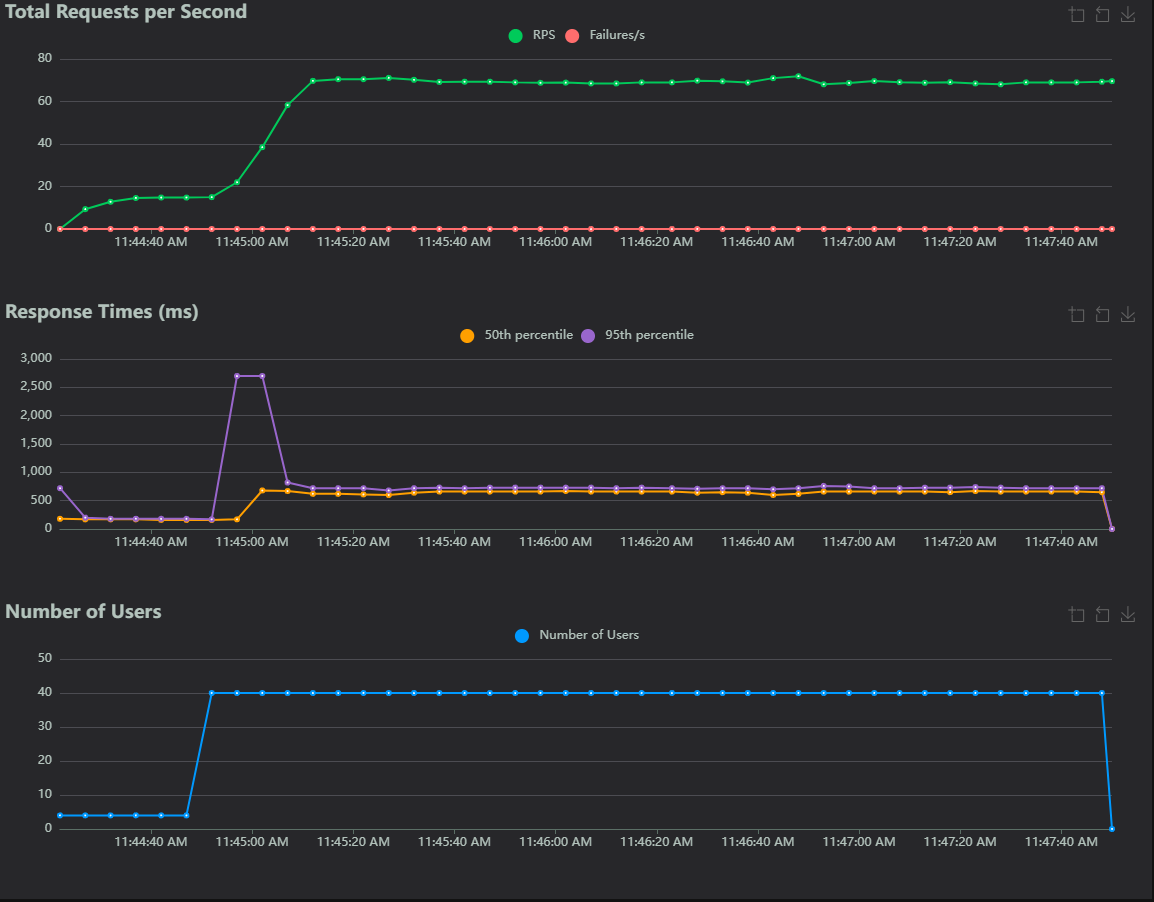
\includegraphics[width=\linewidth]{"figures/hhA - Charts.png"}
  \caption{Very Heavy A --- Locust charts: RPS rises to a \(\sim\)60--70 plateau; percentiles stabilize after WU.}
\end{figure}

\begin{figure}[h!]\centering
  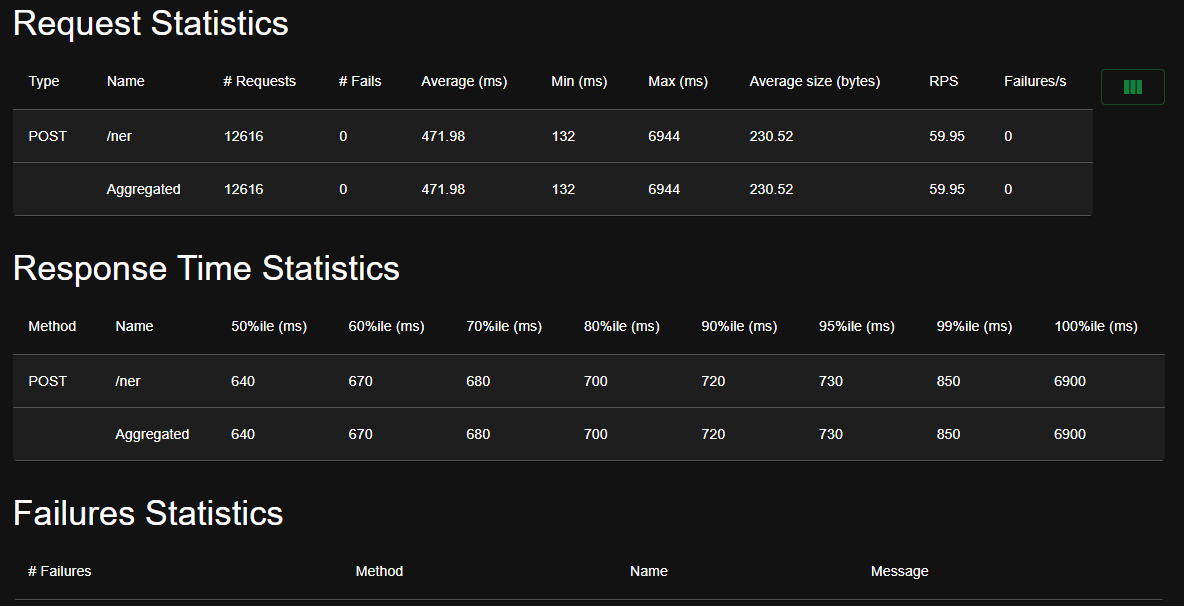
\includegraphics[width=\linewidth]{"figures/hhA - Stats.png"}
  \caption{Very Heavy A --- Locust request statistics (entire run): \#Requests \(\approx\) 12{,}616, p50 \(\approx\) 640\,ms, p95 \(\approx\) 730\,ms, failures \(=0\).}
\end{figure}

\emph{Comparison vs the earlier A runs.} Relative to the previous ``Heavy A'' (10 users, shorter window), hhA sustains a much higher RPS while keeping p95 in the same sub-second band. This indicates that the system still operates below provider-side limits (no visible throttling) and that latency scales gracefully under a higher arrival rate once the function is warm. In CloudWatch, the \texttt{ConcurrentExecutions} curve for hhA (not shown here) reaches a higher, flatter plateau consistent with the new RPS, while \texttt{Duration} remains within a tight band, mirroring the Locust percentiles. Overall, hhA confirms additional headroom beyond the initial ``Heavy A'' envelope.

\section{Limitations and Future Work}


\section{Conclusion}\label{sec:conclusion}

We evaluated a serverless NER API on AWS Lambda behind API Gateway using three canonical workload shapes (A: bursty, B: ramp–steady–ramp, C: spike), each in \emph{Light} and \emph{Heavy} variants, plus targeted vertical scaling experiments. Tests followed the guidance in the performance-evaluation lecture: a short warm-up (WU) to amortize cold starts; a main measurement window with stable load; and both user-facing (Locust) and provider-facing (CloudWatch) metrics. Additional very-heavy scenario ``hhA'' (40 users, low pacing) was executed with a shortened 3-minute plan to probe headroom while staying within budget.

\paragraph{Scalability and efficiency.}
Across all shapes, the service scales cleanly until it approaches the effective concurrency/RPS envelope of the account. Moving from Light \(\rightarrow\) Heavy increases the steady-state RPS while keeping p95/p99 latencies in a narrow, sub-second band once warm. The very-heavy hhA run sustains \(\sim\)60--70~RPS at p95 \(\sim\)0.73\,s with zero failures, demonstrating substantial headroom beyond the initial heavy runs. CloudWatch confirms that \emph{ConcurrentExecutions} rises to a stable plateau commensurate with the higher arrival rate, \emph{Invocations} grow linearly during the steady window, and \emph{Duration} remains stable after WU—indicating the function is CPU/memory provisioned adequately for the tested loads.

\paragraph{Effect of vertical scaling.}
Repeating Heavy\,B at 512\,MB vs.\ 1024\,MB isolated memory’s impact: higher memory (and thus CPU share) reduced p95/p99 latencies and raised sustainable RPS under identical client pacing. This is consistent with Lambda’s proportional CPU\:/\!memory model and shows that vertical scaling is an effective lever when bounded by per-invocation compute rather than by account concurrency.

\paragraph{Workload-shape sensitivity.}
The RU/S/RD structure in B and the transient spike in C produce brief, expected percentile spikes at transitions; the system stabilizes quickly in the steady segment with no persistent oscillations. Light variants are useful to demonstrate stable behavior under realistic pacing, while heavy variants establish the throughput envelope. hhA extends A’s envelope and confirms that higher client concurrency can be accommodated without loss of stability or availability.

\paragraph{Availability and errors.}
No sustained errors or throttles were observed in Locust or CloudWatch during the steady windows. Availability therefore remained effectively \(> 99.9\%\) for the windows considered; brief spikes during transitions are attributed to cold-starts or step changes and do not persist.

\paragraph{Cost awareness.}
Shorter runs (WU 30--60\,s; 2--5\,min main window) and reuse of the same stack kept cost minimal while still yielding statistically meaningful windows, aligning with the budget constraints of the Learner Lab.

\paragraph{Overall.}
Within the tested limits, the architecture \emph{scales accordingly and efficiently}: throughput increases with client concurrency, latency remains controlled and predictable after warm-up, and vertical scaling via memory provides a clear performance uplift when needed. The system shows no anomalous behavior under bursty, ramped, or spiky demand, and maintains zero-failure operation at the highest tested loads (hhA).


\section*{Reproducibility \& Repository Notes}
The repository is organized for ``clone $\rightarrow$ run'' on Windows:
\begin{enumerate}[leftmargin=1.3em]
  \item Install Python 3.10+, Docker Desktop, AWS CLI v2, AWS SAM CLI.
  \item \texttt{python -m venv .venv; . .\textbackslash .venv\textbackslash Scripts\textbackslash Activate.ps1}
  \item \texttt{pip install -r requirements.txt}
  \item \texttt{sam build --use-container}
  \item \texttt{sam deploy --guided --profile learnerlab}
  \item Use \texttt{scripts/smoke.ps1} to POST \texttt{/ner}.
  \item Tear down with \texttt{scripts/delete.ps1}.
\end{enumerate}

\section*{Ethical, Cost, and Budget Considerations}
We designed for negligible standing cost and minimal environmental impact: no always-on compute, small artifacts, and conservative logs. Load tests remain moderate to avoid unintended denial-of-service behavior and unnecessary spend.

\begin{thebibliography}{9}
\bibitem{spacy}
ExplosionAI. \emph{spaCy}. \url{https://spacy.io/}.

\bibitem{NER}
ExplosionAI. \emph{NER in spaCy}. \url{https://spacy.io/api/entityrecognizer}.

\bibitem{sam}
AWS. \emph{AWS Serverless Application Model (SAM)}. \url{https://docs.aws.amazon.com/serverless-application-model/latest/developerguide/}.

\bibitem{lambda}
AWS. \emph{AWS Lambda Developer Guide}. \url{https://docs.aws.amazon.com/lambda/latest/dg/welcome.html}.

\bibitem{apigw}
AWS. \emph{Amazon API Gateway HTTP APIs}. \url{https://docs.aws.amazon.com/apigateway/latest/developerguide/http-api.html}.

\bibitem{cloudwatch}
AWS. \emph{Amazon CloudWatch Metrics for Lambda}. \url{https://docs.aws.amazon.com/lambda/latest/dg/monitoring-metrics.html}.

\bibitem{locust}
Locust. \emph{A modern load testing framework}. \url{https://locust.io/}.
\end{thebibliography}

\end{document}
